\documentclass[UTF8]{ctexart}
\usepackage{amsmath}
\usepackage{diagbox}
\usepackage{textcomp}
\usepackage{graphicx}
\usepackage{float}
\usepackage{caption}
\usepackage{adjustbox}
\usepackage{subfigure}
\usepackage{geometry}
\usepackage{pifont}
\usepackage{chngpage}
\usepackage{bm}
\begin{document}
\renewcommand{\thefootnote}{\fnsymbol{footnote}}
\newgeometry{left=2.5cm,bottom=4cm,right=2.5cm}
%\pagestyle{plain}
\linespread{1.4}
\title{\vspace{-5em}\heiti基于FPGA的简易计算器实验报告\vspace{-2.5em}}
\date{}
\maketitle
\begin{center}
{\fangsong 徐浩博\quad 软件02\quad2020010108}
\end{center}

\subsubsection*{摘要}
{\kaishu\normalsize  本实验旨在通过Verilog硬件语言编写简易计算器代码,并在FPGA上实现,使我们掌握FPGA、Quantus II、Verilog等硬件编程语言和实验软件的使用方法,并且进一步常用组合逻辑电路模块,如选择器、译码器等的概念及应用等知识,并使我们初步掌握了自顶而下的电路设计方法和自底而上的实现方法.}
\subsubsection*{关键词:Quartus II\quad Verilog\quad FPGA\quad 简易计算器 \quad 译码器\quad 四选一选择器\vspace{1.5em}}
\songti

\section{实验仪器}
安装Quartus II的计算机\par
FPGA板\par
适配FPGA板的电源线、数据线
\par

\section{实验内容}
首先我们考虑
\subsection{自顶向下的电路设计}
第一步:对于两个输入的数,我们用加法器add32、减法器sub32、乘法器mul16、除法器div32分别运算出计算结果,结果分别为addans、subans、mulans、divans;这里还需注意,减法器还会输出一个结果的符号sign,其中sign=1表示结果为负,反之为正. 然后我们还需要将四个答案输入四选一选择器selector,同时输入选择的操作operator(两个二进制数,已经由题目规定),选择出该操作对应的运算结果,结果为generalans.\par
第二步:我们需要结合时序逻辑电路,依次快速扫描各个数码管. 首先我们将输入的40MHz时钟信号CLK通过clock模块分频,转化为500Hz的CLK$\_$信号;然后我们在CLK$\_$的每个上升沿来临时使得计数器wordselector加一. wordselector实际表示第几个数码管选通,因此选通的数码管编号就能以500Hz的频率切换. 我们将选定的数码管编号通过译码器,转化为位选信号并输出,这样就可以指定好当前选通的数码管,同时选定的数码管编号还将以500Hz的频率切换,达到扫描的目的.\par
第三步:我们还需要获得当前选定的数码管应该显示的内容,也即获得段选信号. 我们将第一步获得的总答案generalans和符号显示signout(sign=1且operator=10,也即当前运算为减法且计算结果为负数时signout=1, 方显示负号),还有第二步获得的选通的数码管编号全部输入gettempnumber内,获得当前数码管应该输出的数字;最后将该数字经过numbertranslator的七段译码器后,输出真正的数码管段选信号.
\begin{figure}[H]\begin{center}
    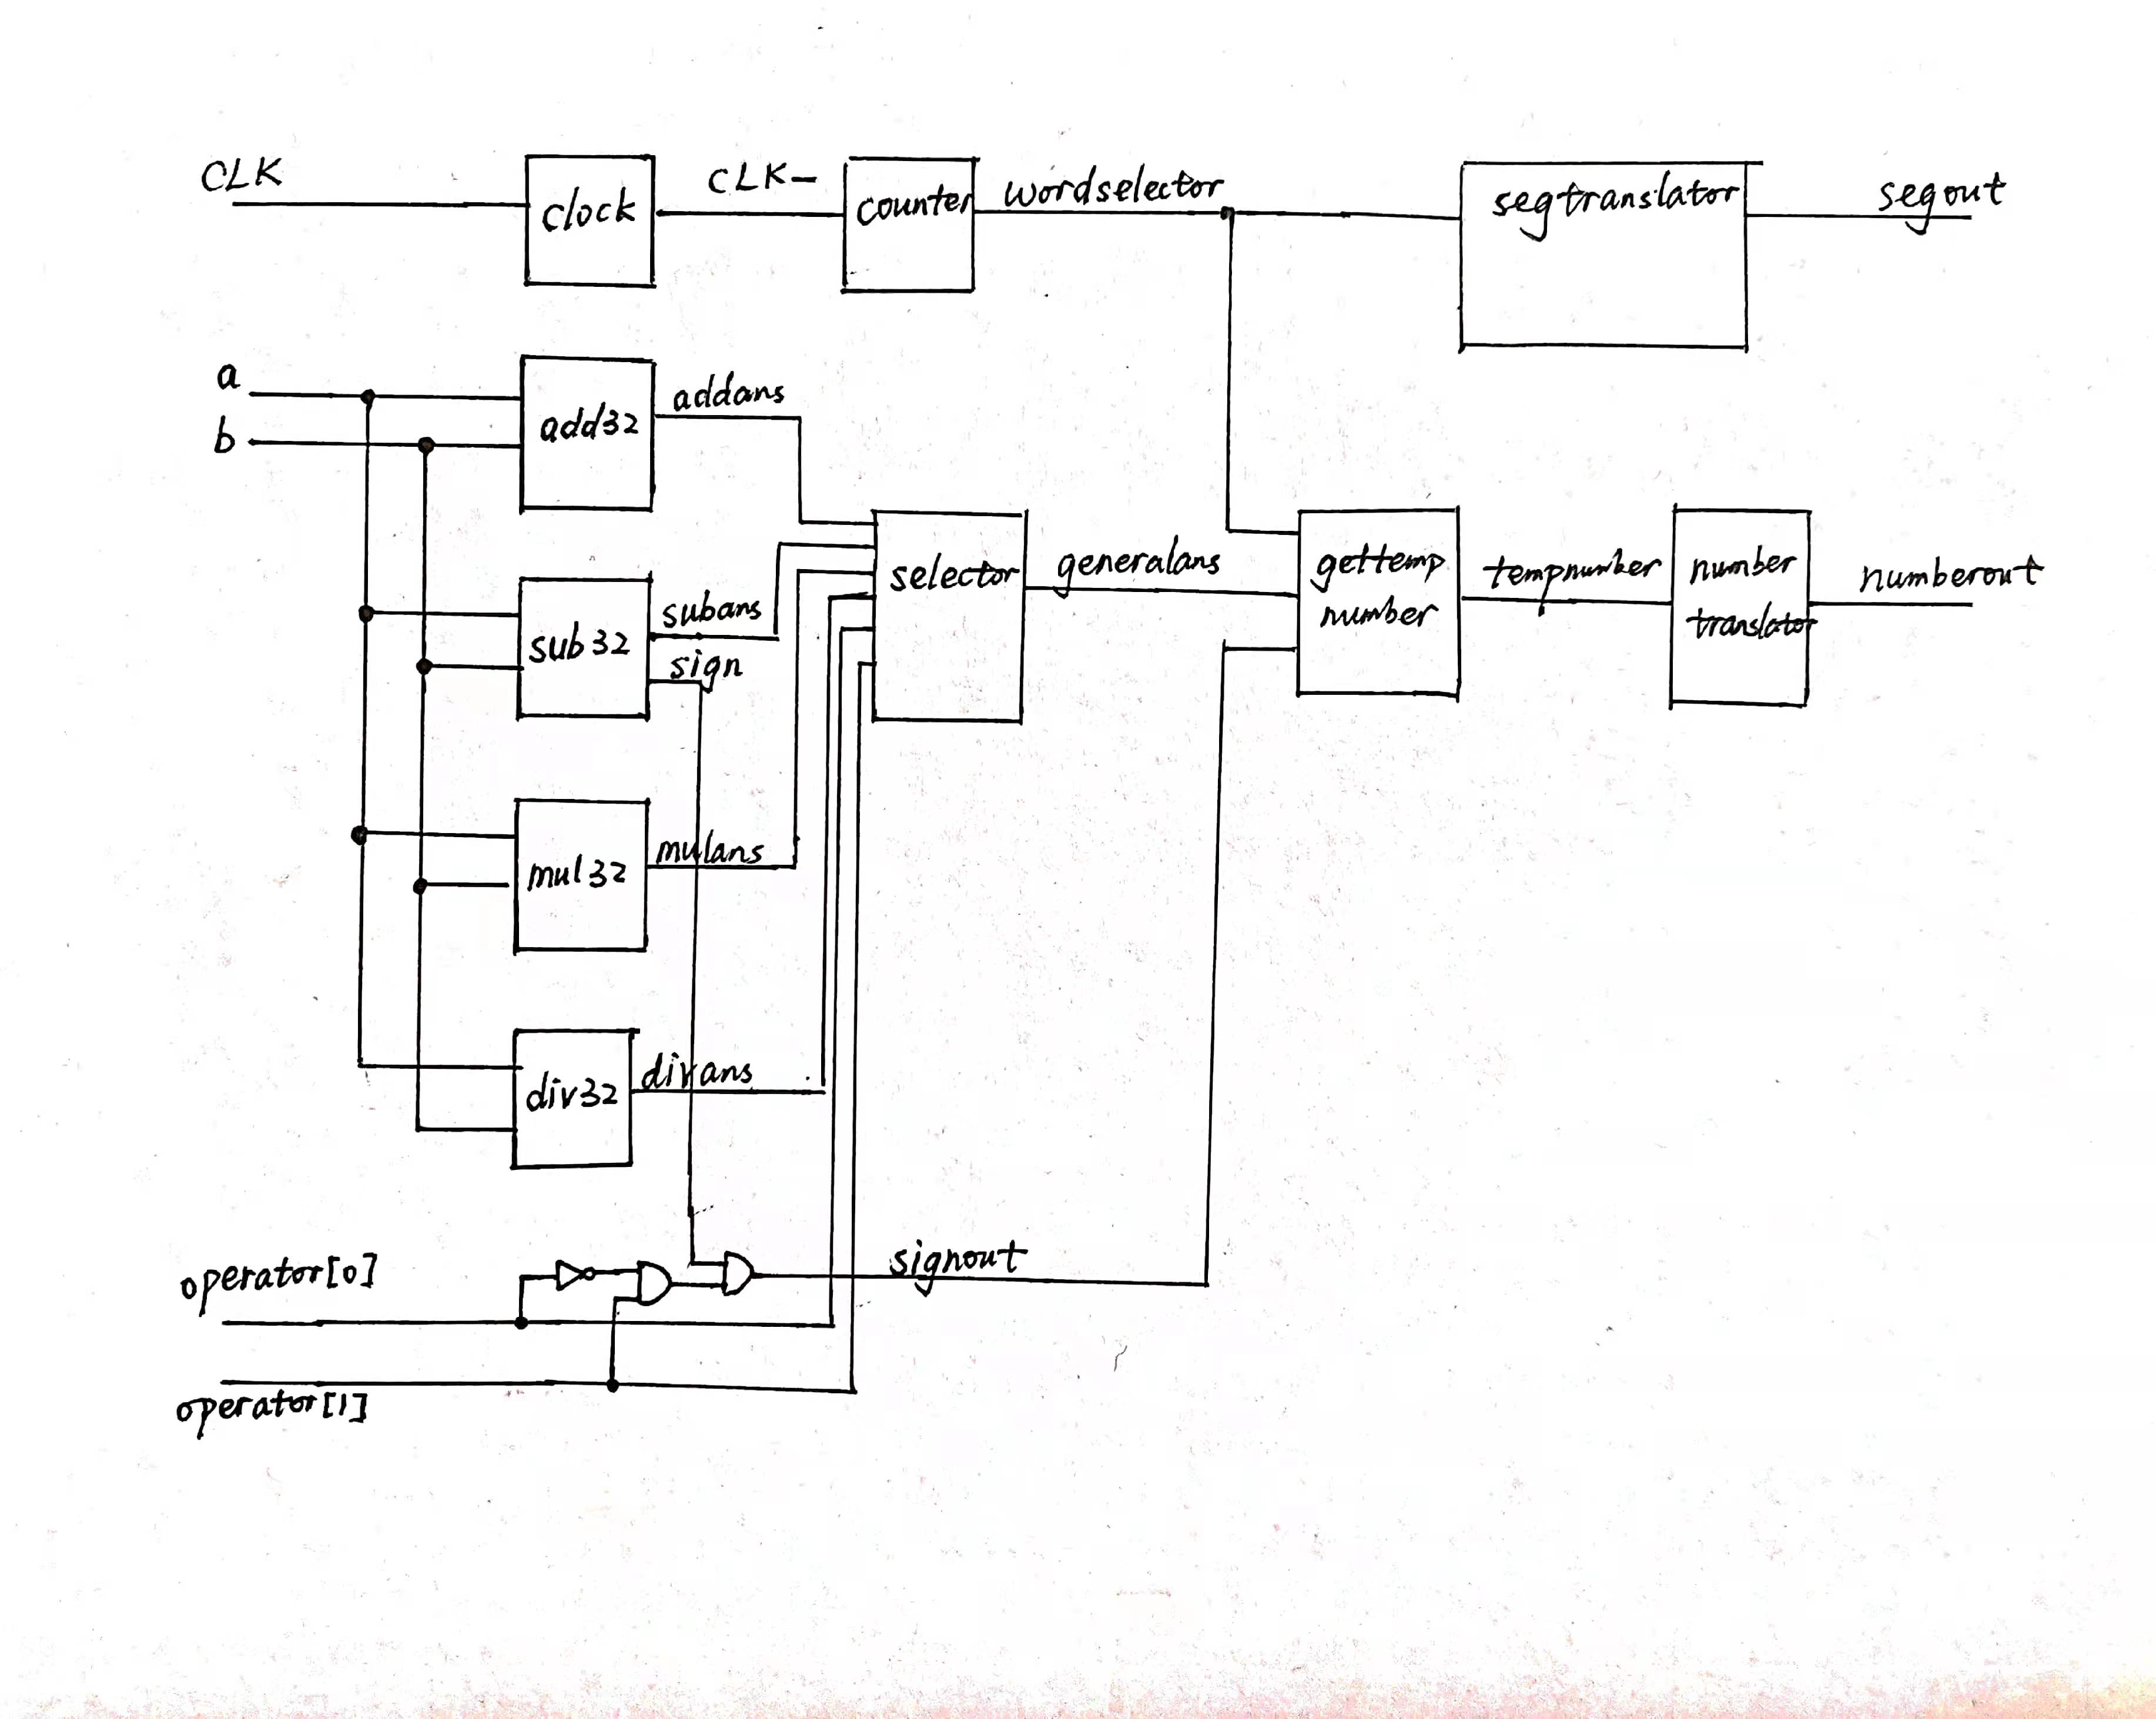
\includegraphics[scale=0.12]{1.jpg}
\end{center}\end{figure}
\subsection{自底向上的电路设计}
\subsubsection{第一步的内容}

对于第一步的内容,我们需要实现四个运算器和一个四选一选择器,每个模块具体如下:\\
\paragraph{加法器add32}:\par
输入:运算数a,b\par
输出:两数之和addans
\begin{figure}[H]\begin{center}
    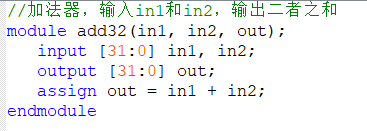
\includegraphics[scale=1]{add32.PNG}
\end{center}\end{figure}
\paragraph{乘法器mul16}:\par
输入:运算数a,b\par
输出:两数之积mulans
\begin{figure}[H]\begin{center}
    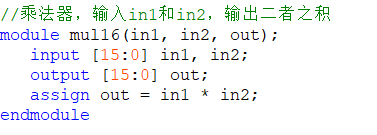
\includegraphics[scale=1]{mul16.PNG}
\end{center}\end{figure}
\paragraph{除法器div32}:\par
输入:运算数a,b\par
输出:两数之比divans
\begin{figure}[H]\begin{center}
    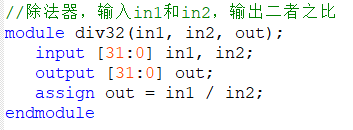
\includegraphics[scale=1]{div32.PNG}
\end{center}\end{figure}
\paragraph{减法器sub32}:\par
输入:运算数a,b\par
输出:两数之差subans和运算符号sign(sign=1为负,反之为正)\par
具体实现:在运算完subans=a-b后,需要用always过程为sign赋值;当a>=b时sign=0,否则sign=1,这样就获得了运算符号sign的输出结果.
\begin{figure}[H]\begin{center}
    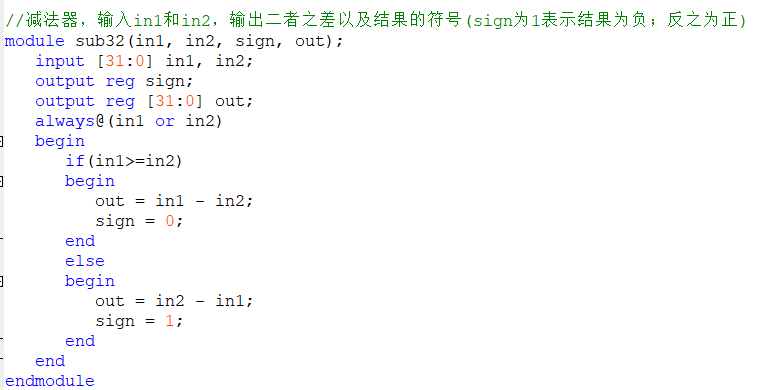
\includegraphics[scale=1]{sub32.PNG}
\end{center}\end{figure}
\paragraph{四选一选择器selector}:\par
输入:四个运算数、选择的运算符号operator\par
输出:四个运算数中的一个generalans\par
具体实现:对operator进行条件判断,对operator的四种可能取值分别讨论,并分别给generalans赋不同的值.
\begin{figure}[H]\begin{center}
    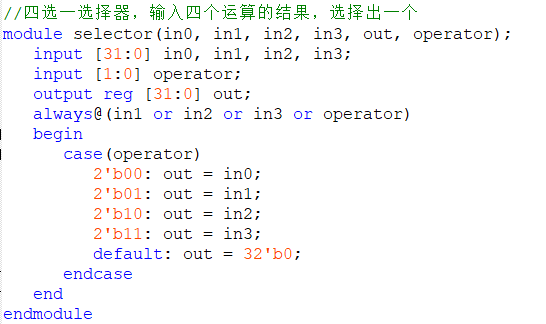
\includegraphics[scale=1]{selector.PNG}
\end{center}\end{figure}

\subsubsection{第二步的内容}

对于第二步的内容,我们需要实现一个分频器、一个位选计数器、一个位选信号译码器,每个模块具体如下:\\
\paragraph{分频器clock}:\par
输入:分频前的时钟信号CLK\par
输出:分频后的时钟信号CLK\_\par
具体实现:通过一个计数器count记录clk的高电平次数,每次clk高电平则count自加一,如此,count[15]的变化频率就应该是clk变化频率的$1/2^{16}$倍,也即频率大约为500Hz. 我们令CLK\_与count[15]变化相同,那么CLK\_的时钟频率就是500Hz了.
\begin{figure}[H]\begin{center}
    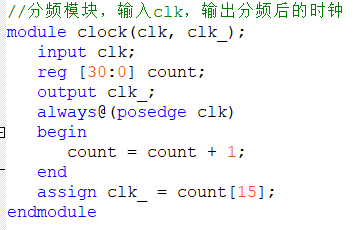
\includegraphics[scale=1]{clock.PNG}
\end{center}\end{figure}
\paragraph{位选计数器counter}:\par
输入:时钟信号CLK\_\par
输出:位选编号wordselector\par


具体实现:每当CLK\_为高电平时,wordselector均会自增1,但考虑到wordselector只有3个二进制位,因此它会以CLK\_的频率在000,001...111,000,001之间变化且循环,那么我们将这样的信号视作信号管编号,就可以实现扫描式位选,输出也即位选的信号管编号.
\begin{figure}[H]\begin{center}
    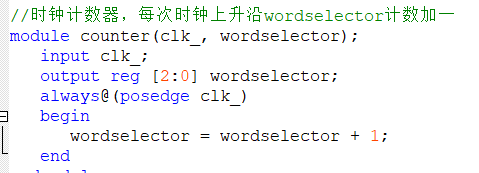
\includegraphics[scale=1]{counter.PNG}
\end{center}\end{figure}

\paragraph{位选信号译码器segtranslator}:\par
输入:位选编号wordselector\_\par
输出:位选信号segout\par
功能表:
设wordselector各位为$A_2,A_1,A_0$,输出为$Y_5-Y_0$
\begin{table}[H]\begin{center}
    \begin{tabular}{c c c|c c c c c c}
        \hline
        $A_2$&$A_1$&$A_0$&$Y_5$&$Y_4$&$Y_3$&$Y_2$&$Y_1$&$Y_0$\\
        \hline
        0&0&0&1&1&1&1&1&0\\
        \hline
        0&0&1&1&1&1&1&0&1\\
        \hline
        0&1&0&1&1&1&0&1&1\\
        \hline
        0&1&1&1&1&0&1&1&1\\
        \hline
        1&0&0&1&0&1&1&1&1\\
        \hline
        1&0&1&0&1&1&1&1&1\\
        \hline
        1&X&X&1&1&1&1&1&1\\
        \hline
    \end{tabular}
    \end{center}\end{table}
具体实现:将位选编号通过条件判断,选中的信号管输出低电平,转化为位选信号[0-5].
\begin{figure}[H]\begin{center}
    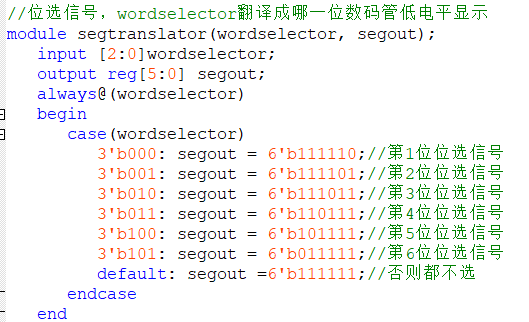
\includegraphics[scale=1]{segtranslator.PNG}
\end{center}\end{figure}

\subsubsection{第三步的内容}

对于第三步的内容,我们需要实现当前数字获取器和一个七段信号管显示译码器,每个模块具体如下:\\
\paragraph{当前数字获取器gettempnumber}:\par
输入:运算数a,b,运算结果generalans,运算结果的符号signout\par
输出:当前数码管应当显示的数字tempnumber\_\par

具体实现:如果当前是第一个数码管显示,那么当前数码管应该显示运算数a,直接将a赋给结果(注意,a为十六进制,译码时需要将数字转化为0-f);如果当前是第二个数码管显示,那么当前数码管应该显示运算数b,直接将b赋给结果. 如果当前是第四/五/六个数码管显示,应该显示运算结果,那么就将十进制运算结果进行相应的运算,并将当前位的数字赋给结果. 需要特别注意的是,如果当前是第三个数码管显示,那么应该显示符号:如果需要显示负号,则结果赋值为-1,表示需要显示为负号,否则结果赋值为-2表示为灭零. 这里的-1,-2都做了特别约定.
\begin{figure}[H]\begin{center}
    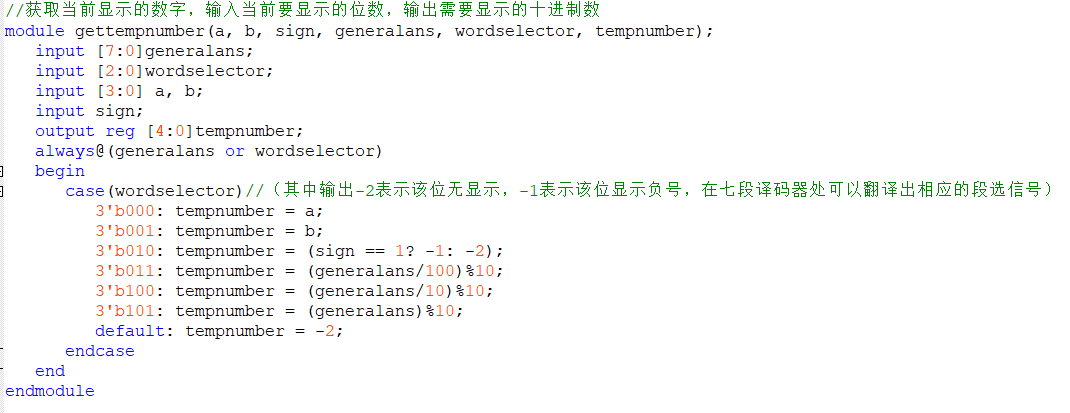
\includegraphics[scale=1]{gettempnumber.PNG}
\end{center}\end{figure}

\paragraph{七段信号管显示译码器numbertranslator}:\par
输入:当前数码管应当显示的数字tempnumber\par
输出:数码管段选信号\par
功能表:
设wordselector各位为$A_4,A_3,A_2,A_1,A_0$,输出为$Y_6-Y_0$
\begin{table}[H]\begin{center}
    \begin{tabular}{c c c c c|c c c c c c c}
        \hline
        $A_4$&$A_3$&$A_2$&$A_1$&$A_0$&$Y_6$&$Y_5$&$Y_4$&$Y_3$&$Y_2$&$Y_1$&$Y_0$\\
        \hline
        0&0&0&0&0&1&0&0&0&0&0&0\\
        \hline
        0&0&0&0&1&1&1&1&1&0&0&1\\
        \hline
        0&0&0&1&0&0&1&0&0&1&0&0\\
        \hline
        0&0&0&1&1&0&1&1&0&0&0&0\\
        \hline
        0&0&1&0&0&0&0&1&1&0&0&1\\
        \hline
        0&0&1&0&1&0&0&1&0&0&1&0\\
        \hline
        0&0&1&1&0&0&0&0&0&0&1&0\\
        \hline
        0&0&1&1&0&1&1&1&1&0&0&0\\
        \hline
        0&0&1&1&1&0&0&0&0&0&0&0\\
        \hline
        0&1&0&0&0&0&0&1&0&0&0&0\\
        \hline
        0&1&0&1&0&0&0&0&1&0&0&0\\
        \hline
        0&1&0&1&1&0&0&0&0&0&1&1\\
        \hline
        0&1&1&0&0&1&0&0&0&1&1&0\\
        \hline
        0&1&0&1&0&1&0&0&0&0&0&1\\
        \hline
        0&1&1&1&0&0&0&0&0&1&1&0\\
        \hline
        0&1&1&1&1&0&0&0&0&1&1&0\\
        \hline
        1&1&1&1&1&0&1&1&1&1&1&0\\
        \hline
        X&X&X&X&X&1&1&1&1&1&1&1\\
        \hline
    \end{tabular}
    \end{center}\end{table}
具体实现:我们通过真值表,对数字对应的段选信号输出进行一一讨论. 需要注意的是,如果输入的数大于9,那么必然不是generalans的某一位,而是a,b中的一个,需要用十六进制输出,将之转化为0-f. 同时,我们已经做了特别约定,-1(5'b11111)对应负号,-2(其他情况default)对应灭零,这些都需要译码器做特殊处理.
\begin{figure}[H]\begin{center}
    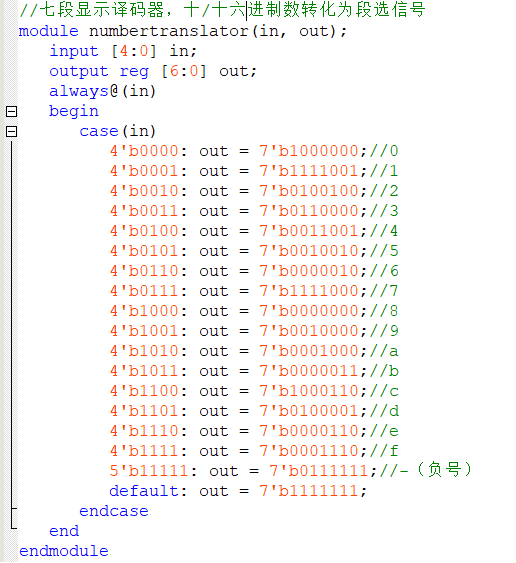
\includegraphics[scale=1]{numbertranslator.PNG}
\end{center}\end{figure}

\subsubsection{组装}
最后,我们还需要将各部分的模块按照自顶向下设计的电路图而组装在一起. 具体组装的代码见下,细节已经在注释中给出:
\begin{figure}[H]\begin{center}
    \newgeometry{left=0em,right=0em}
    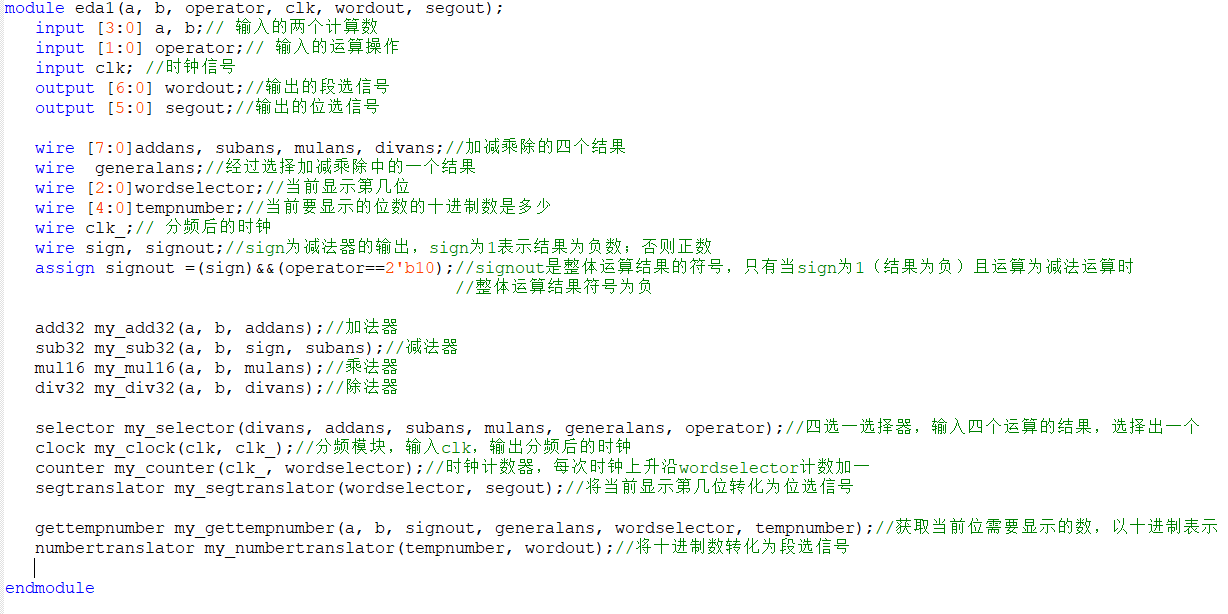
\includegraphics[scale=0.65]{main.PNG}
\end{center}\end{figure}

\section{实现效果展示}
我们首先进行仿真波形验证。1)加法
\begin{figure}[H]\centering
    {
        \newgeometry{a4paper,left=3cm,right=0cm}
        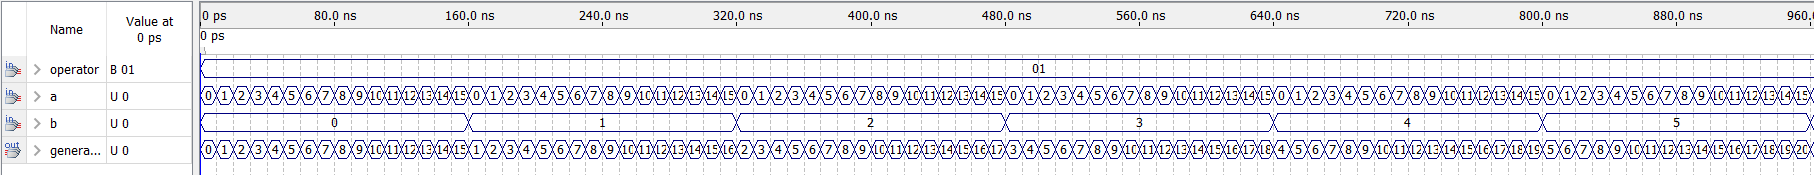
\includegraphics[scale=0.5]{add.PNG}
        \restoregeometry
    }
\end{figure}
    2)加法
    \begin{figure}[H]\centering
        {
            \newgeometry{a4paper,left=3cm,right=0cm}
            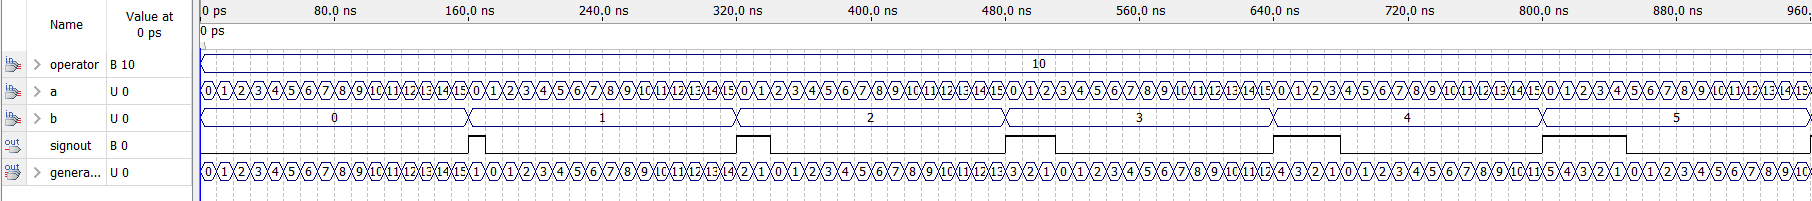
\includegraphics[scale=0.5]{sub.PNG}
            \restoregeometry
        }
    \end{figure}
其中signout是符号位,signout=1表示需要将ans取负号.
3)乘法
\begin{figure}[H]\centering
    {
        \newgeometry{a4paper,left=3cm,right=0cm}
        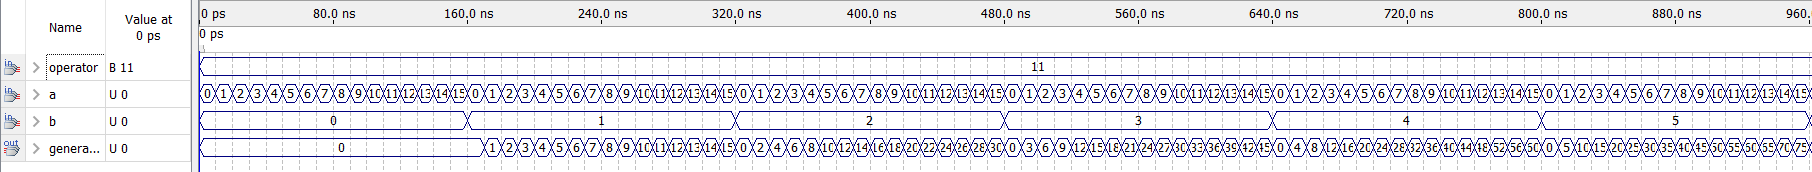
\includegraphics[scale=0.5]{mul.PNG}
        \restoregeometry
    }
\end{figure}

可见运行正确. 最后我们烧制到FPGA板上进行验证.
\begin{figure}[H]\centering
    {
    \newgeometry{a4paper,left=3cm,right=0cm}
    \vspace{-1em}
    \subfigcapskip=-10pt
    \subfigure[1+1=2]{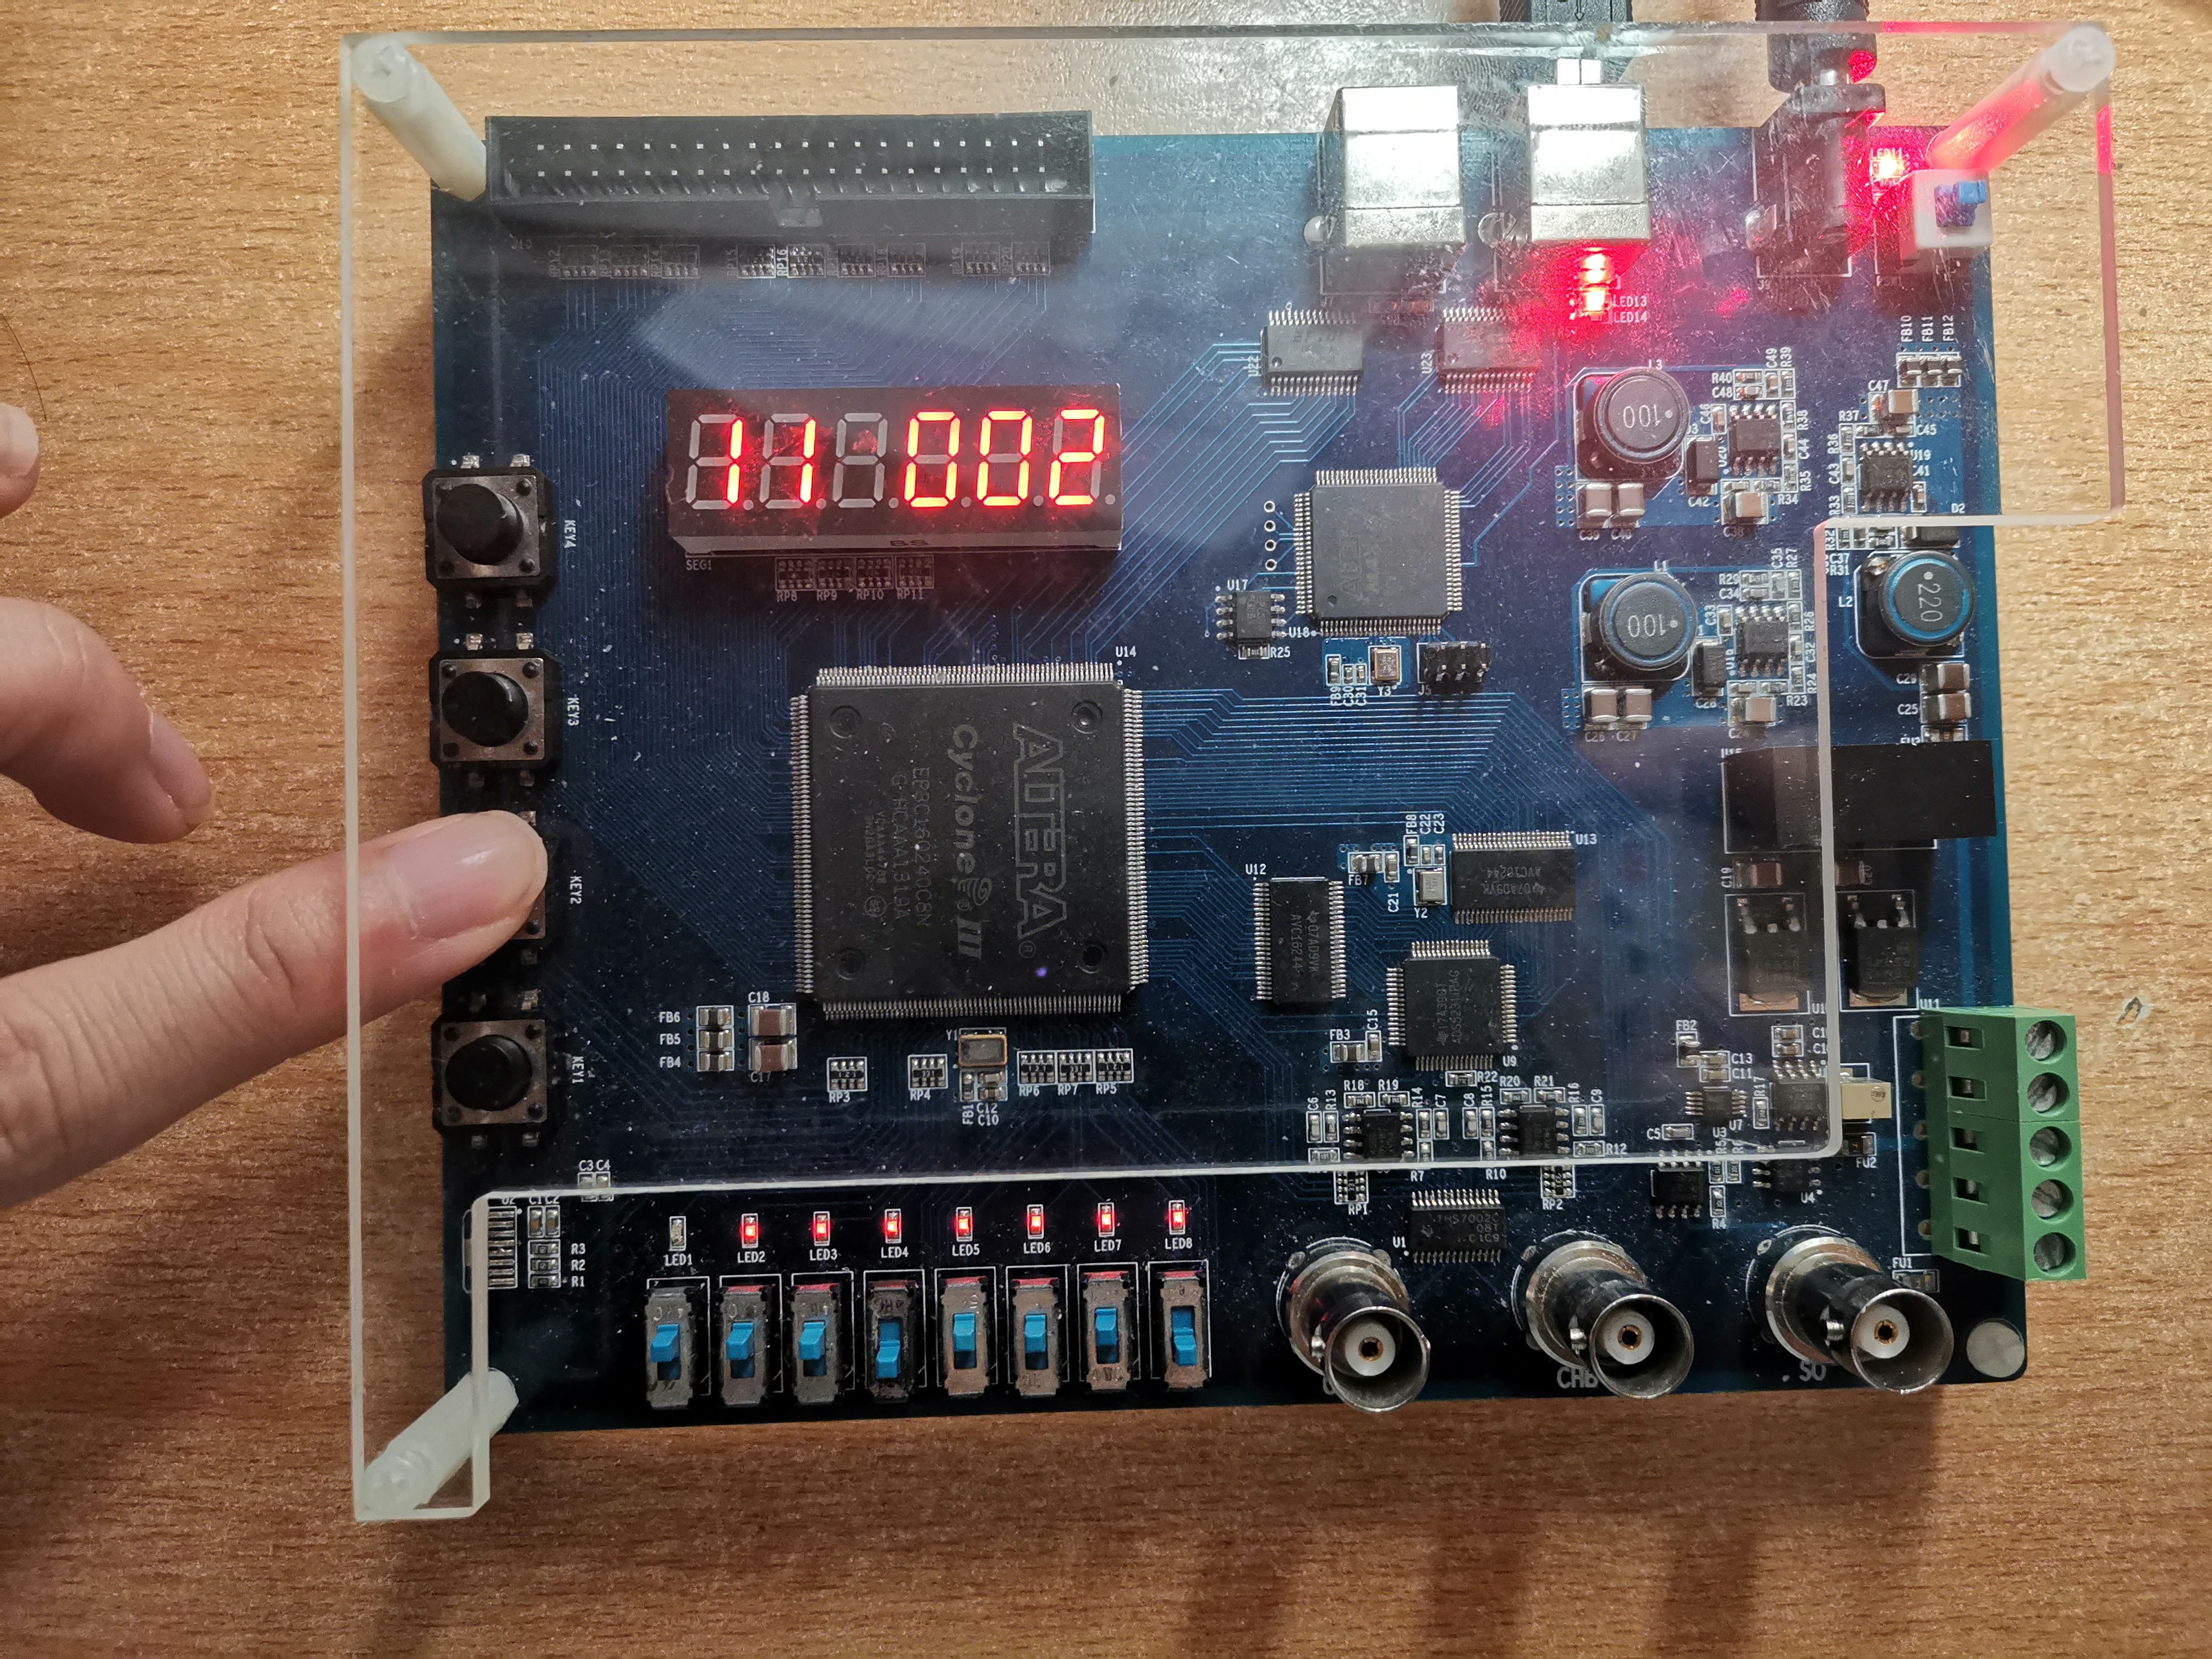
\includegraphics[scale=0.06]{1+1.jpg}}\hspace{0.3mm}
    \subfigure[14+14=28]{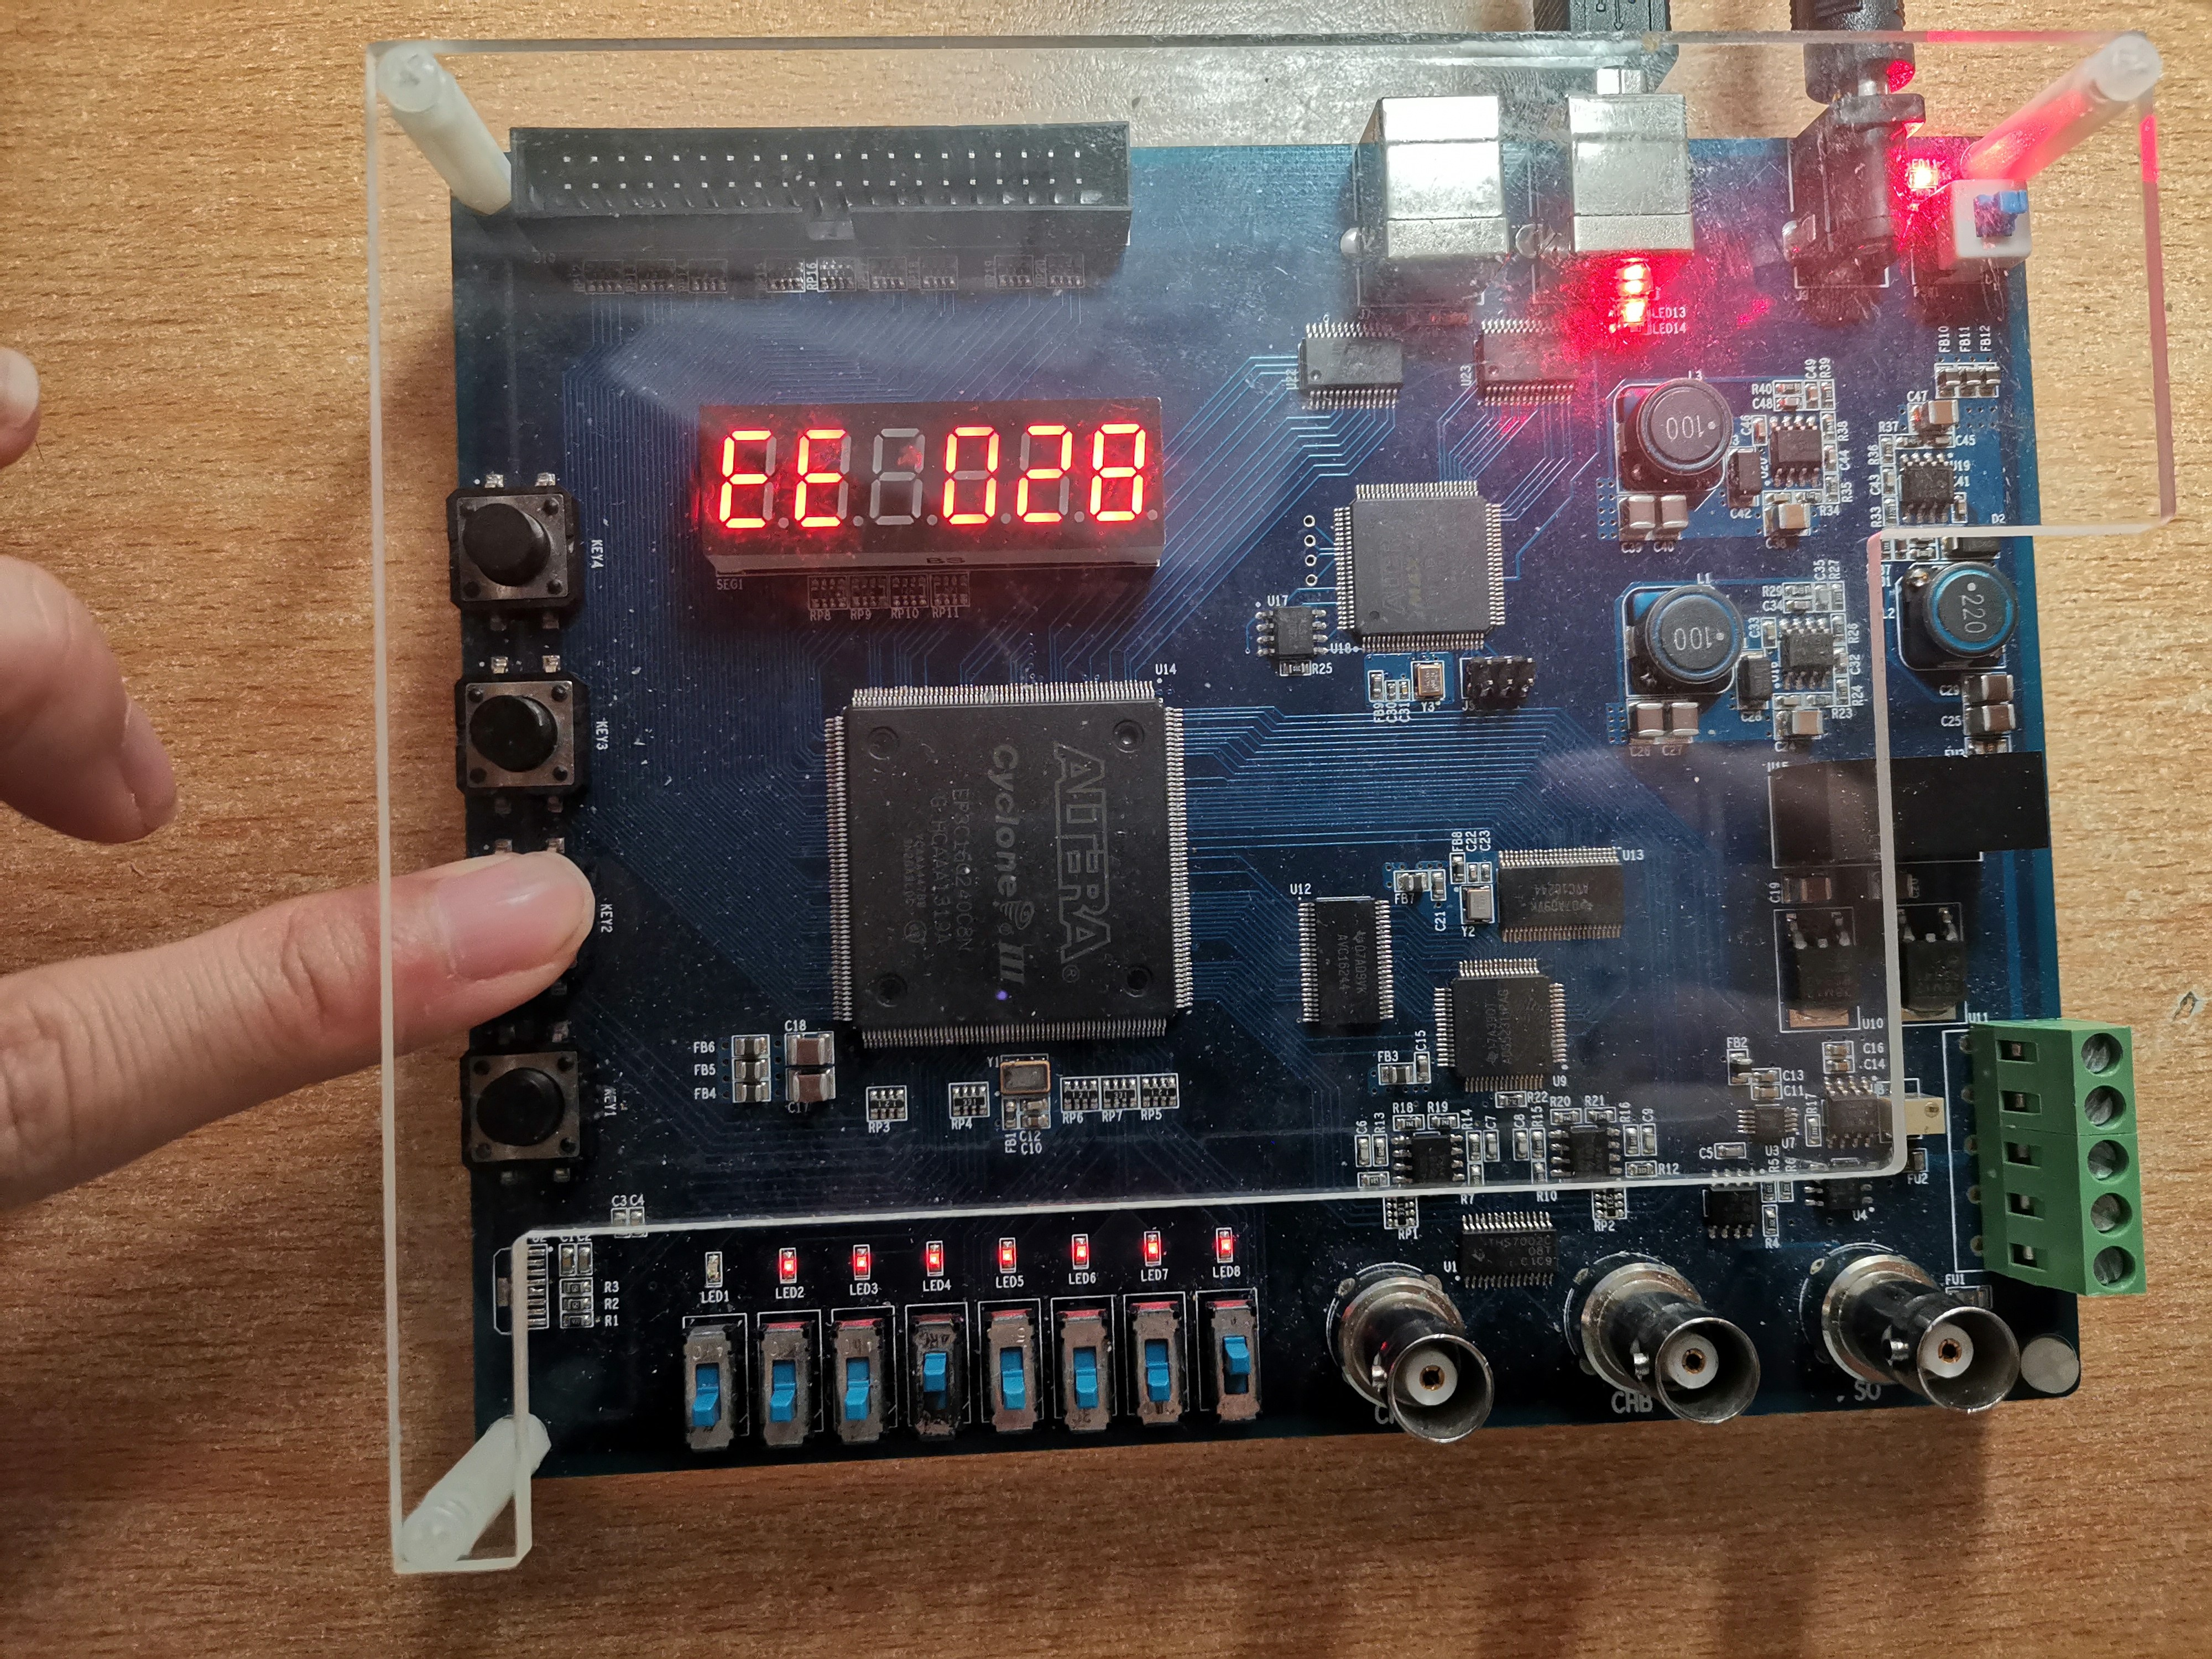
\includegraphics[scale=0.06]{14+14.jpg}}\hspace{0.3mm}
    \subfigure[0-12=-12]{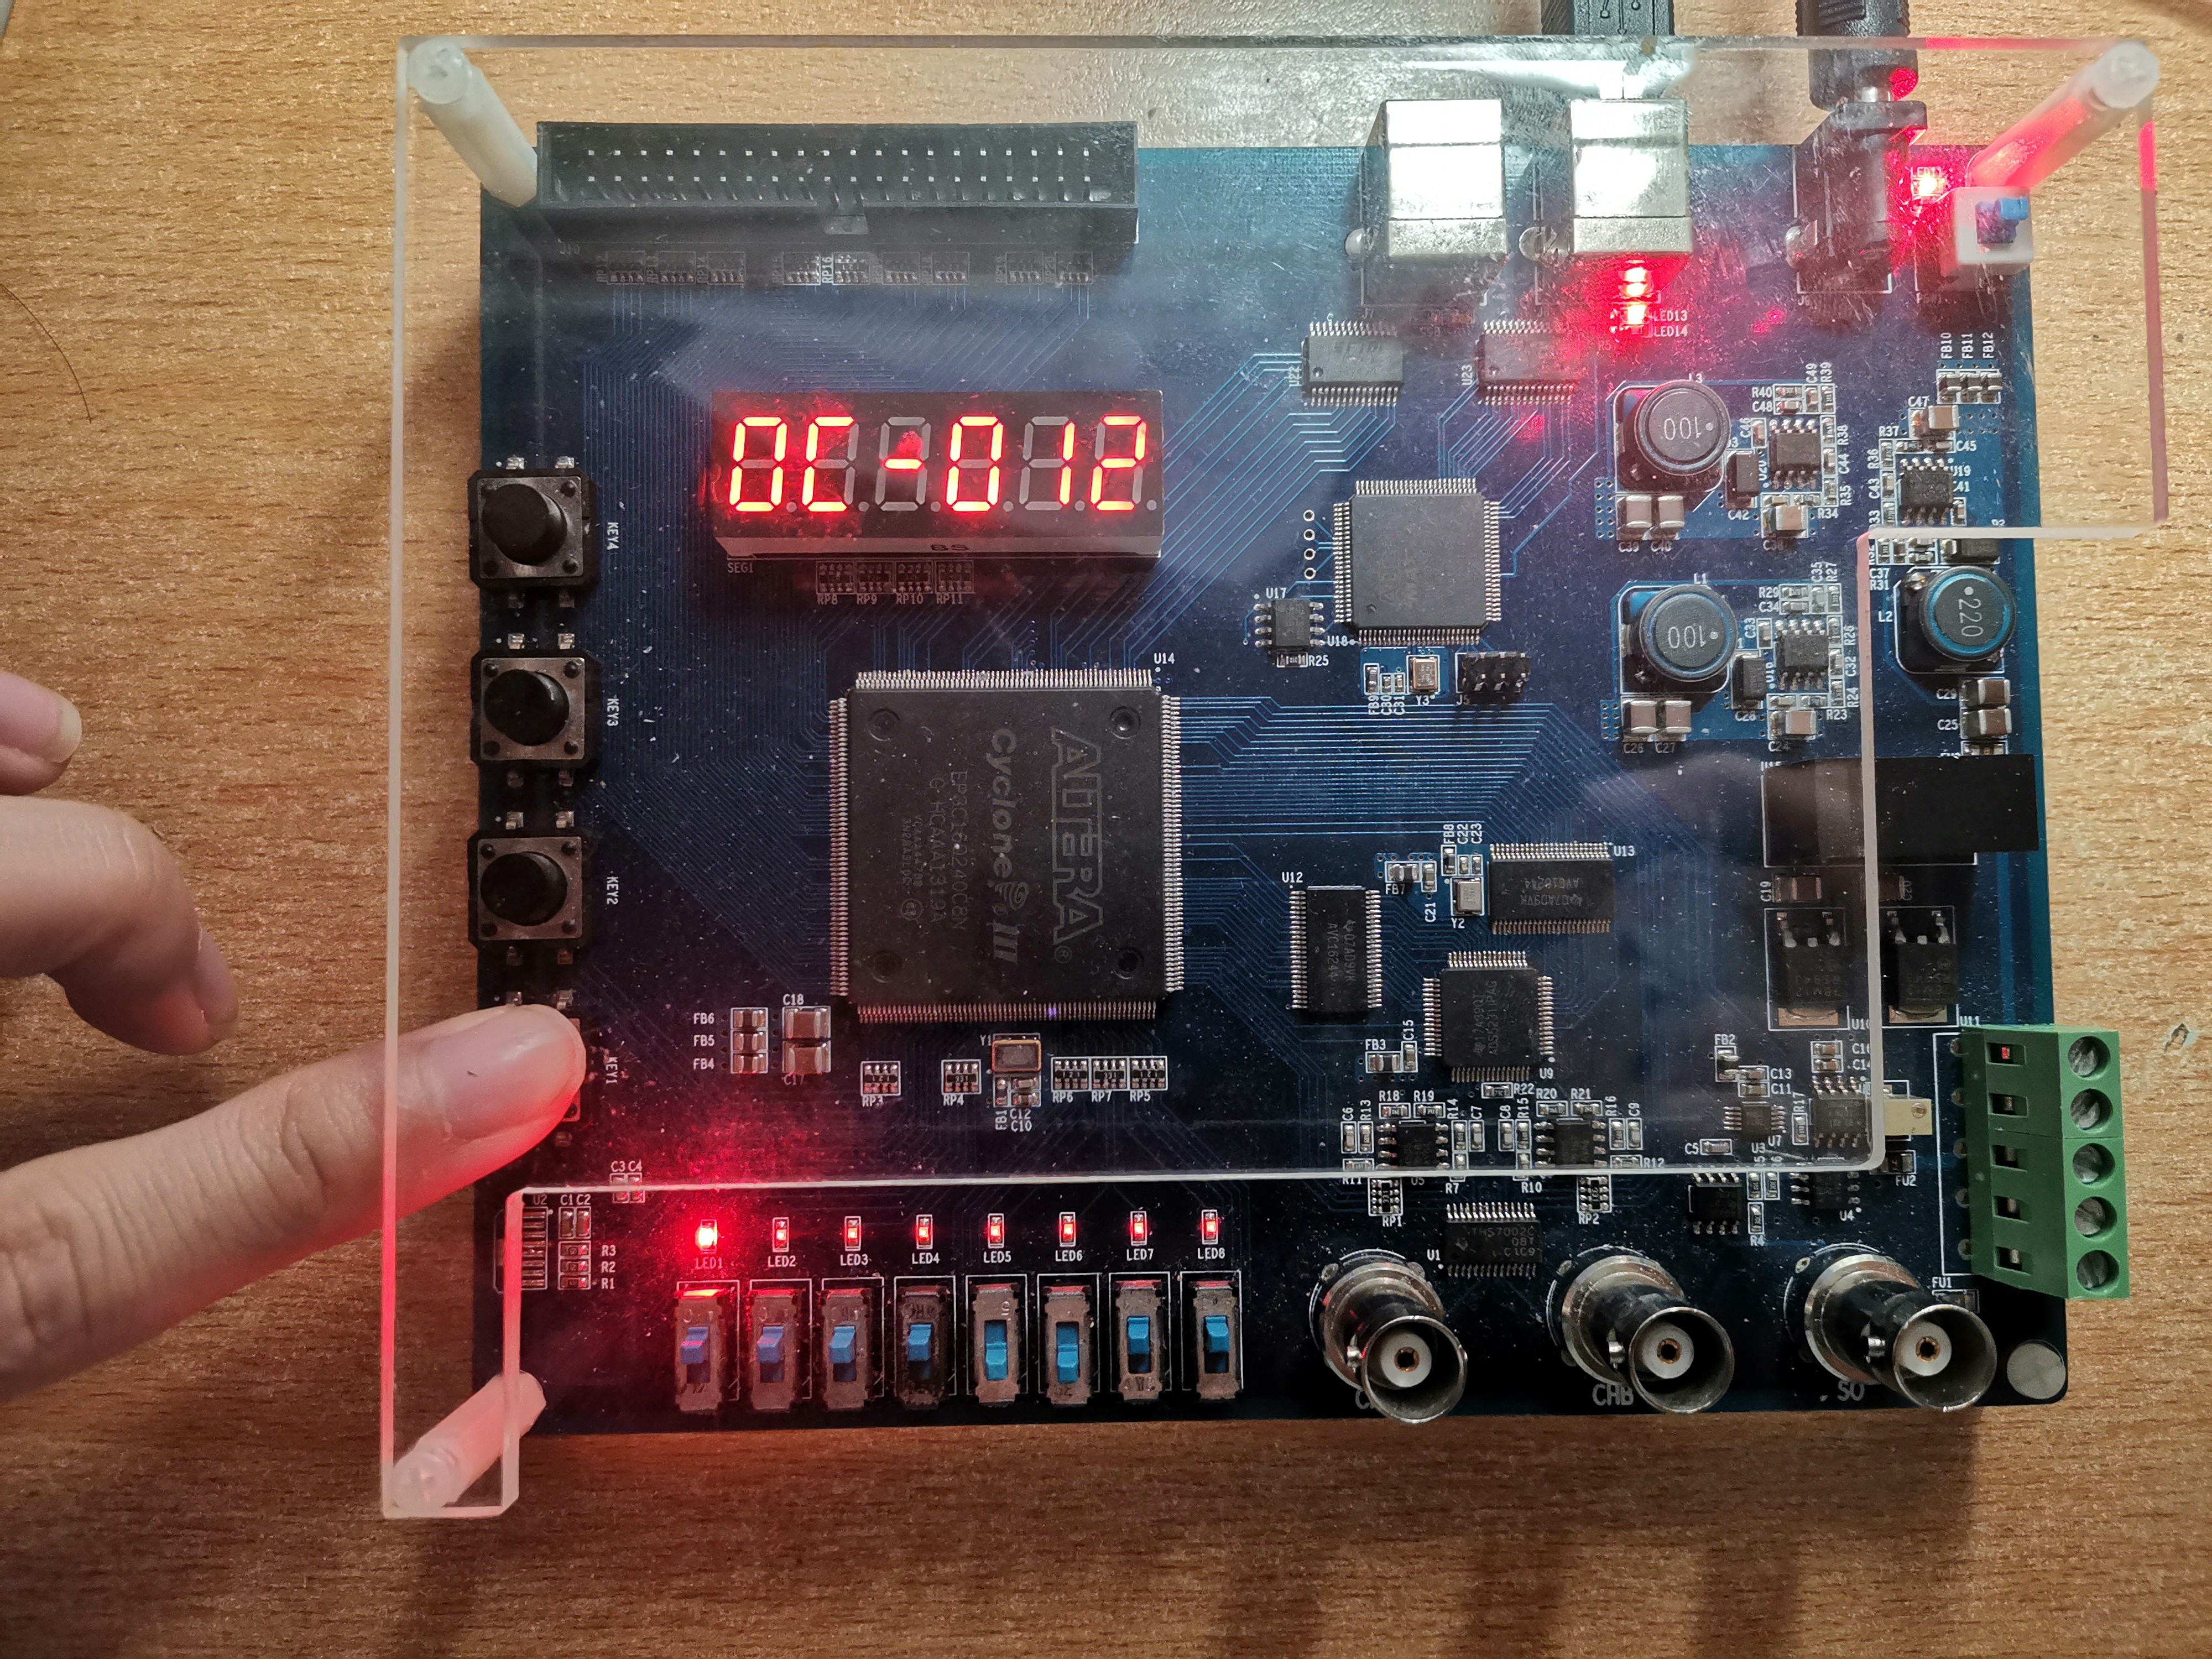
\includegraphics[scale=0.06]{0-12.jpg}}\hspace{0.3mm}
    \subfigure[3-15=-12]{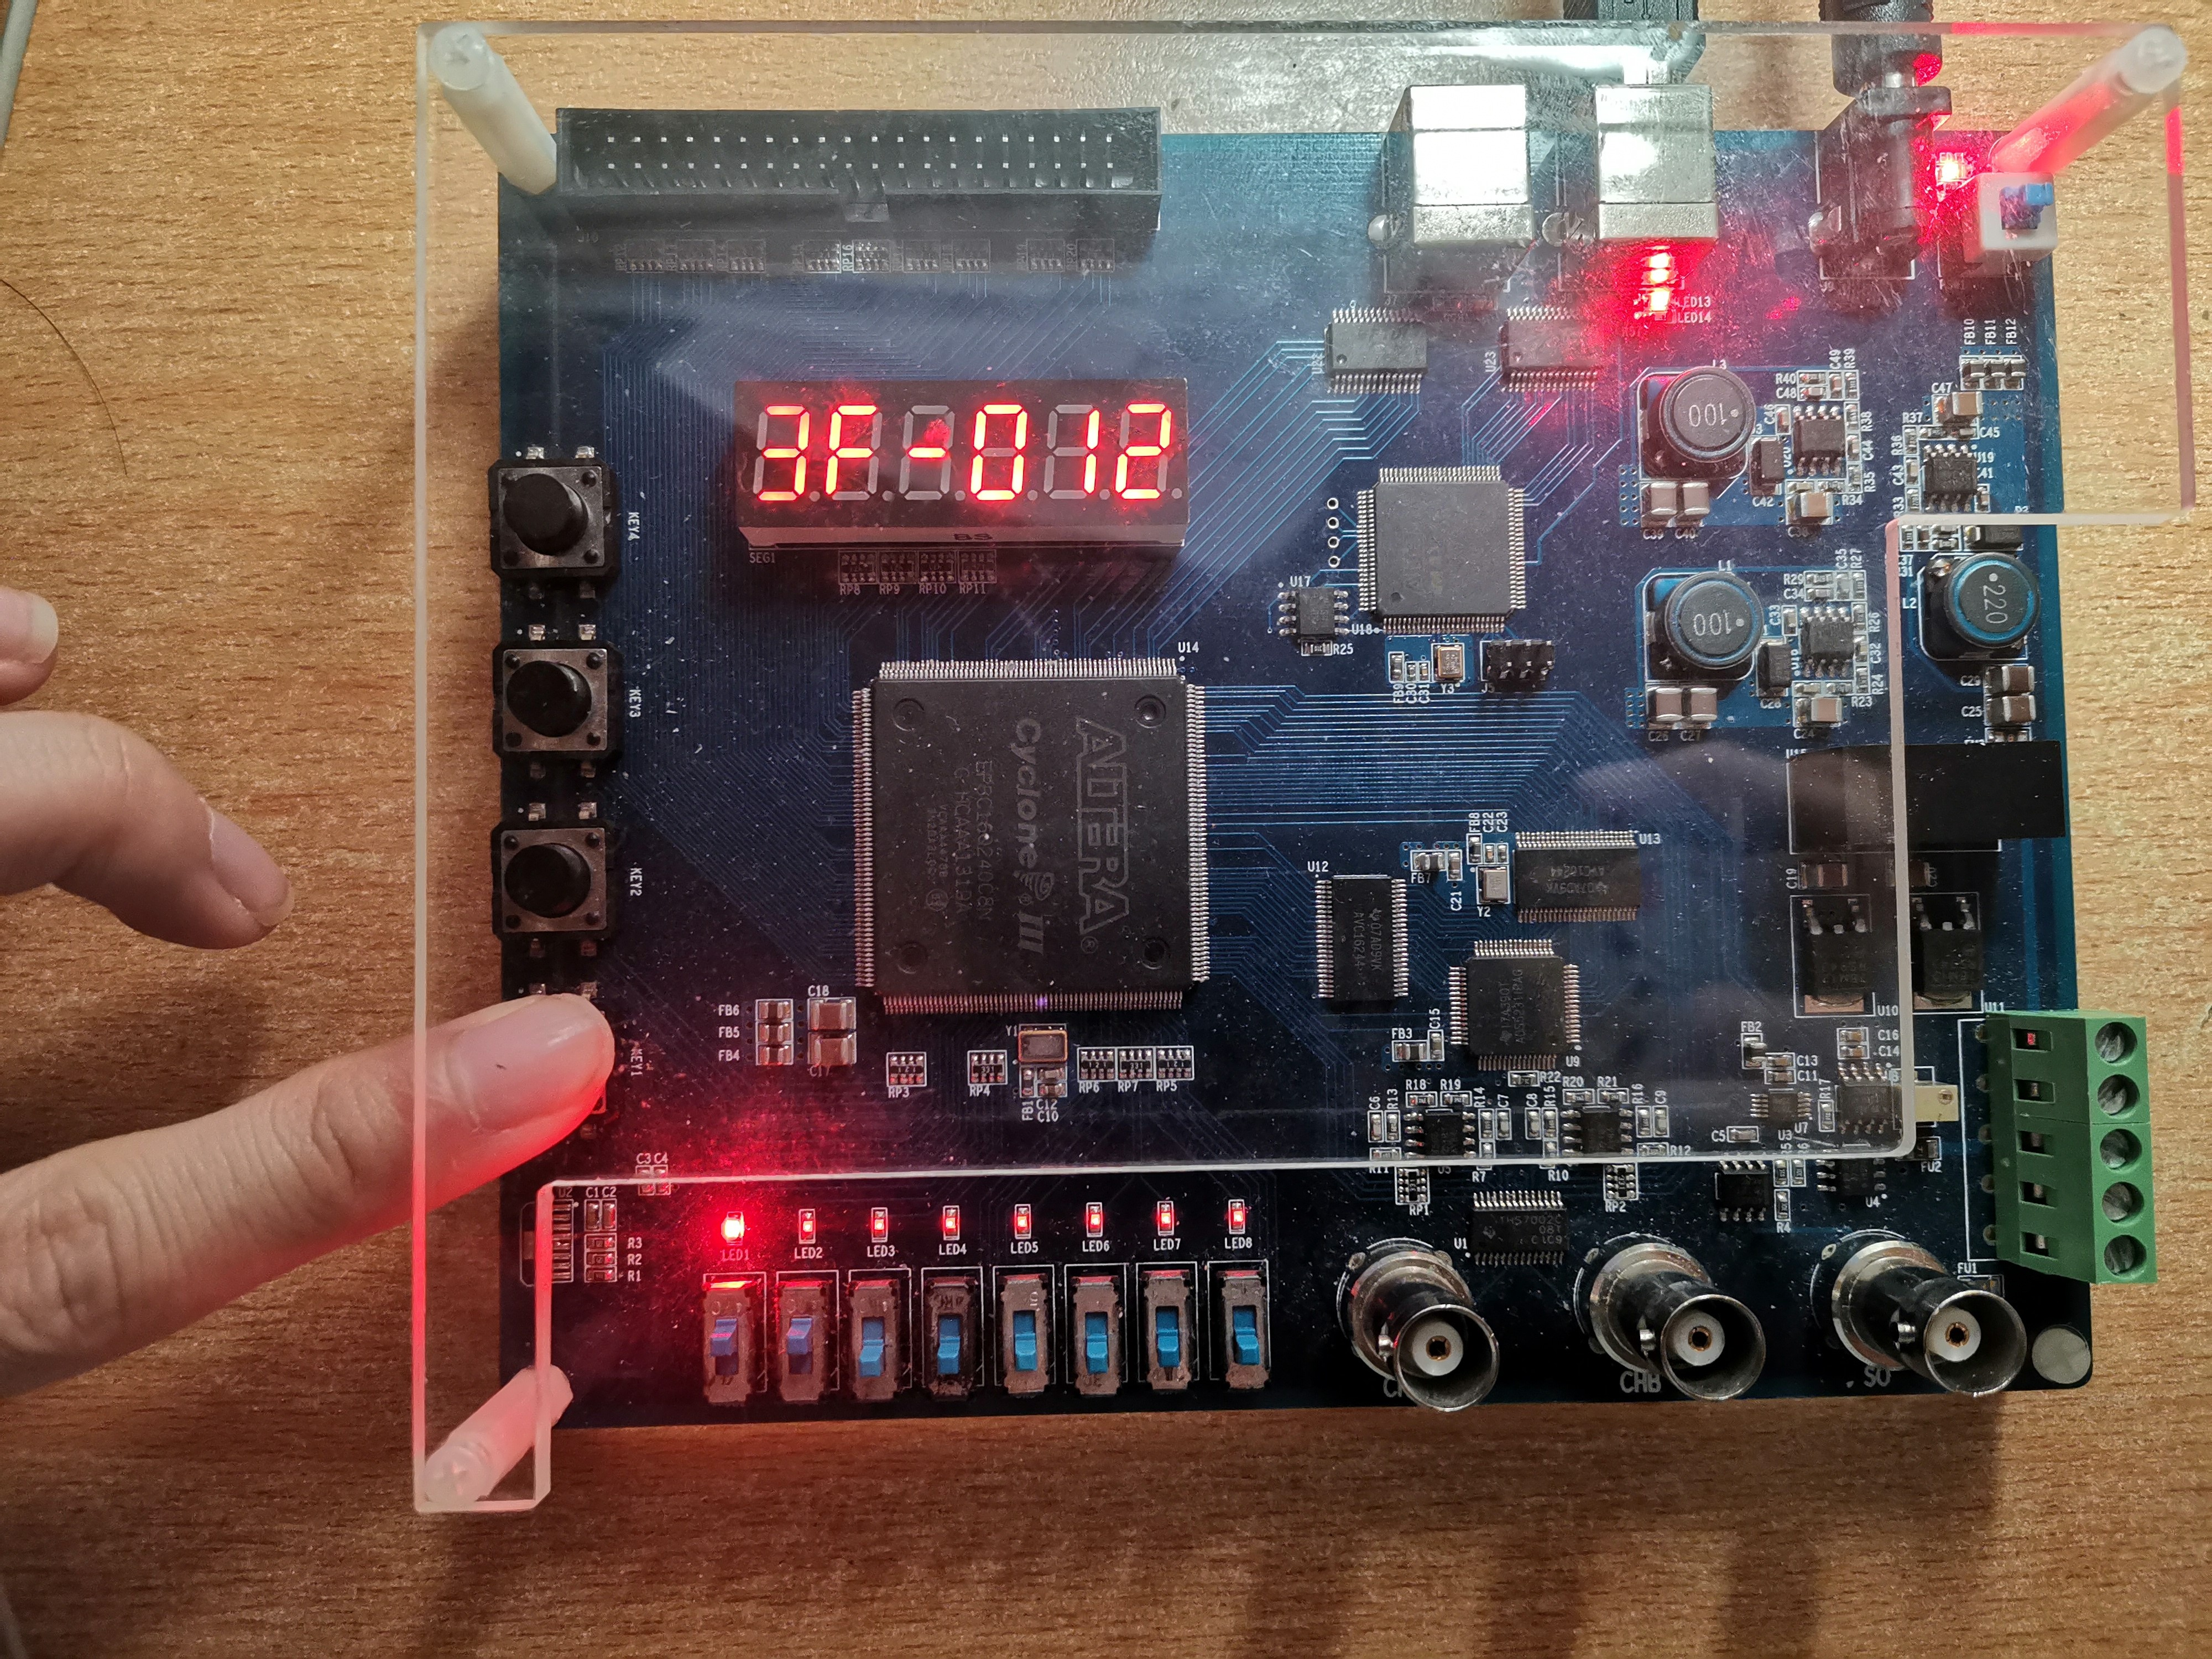
\includegraphics[scale=0.06]{3-15.jpg}}\hspace{0.3mm}
    \subfigure[6×15=90]{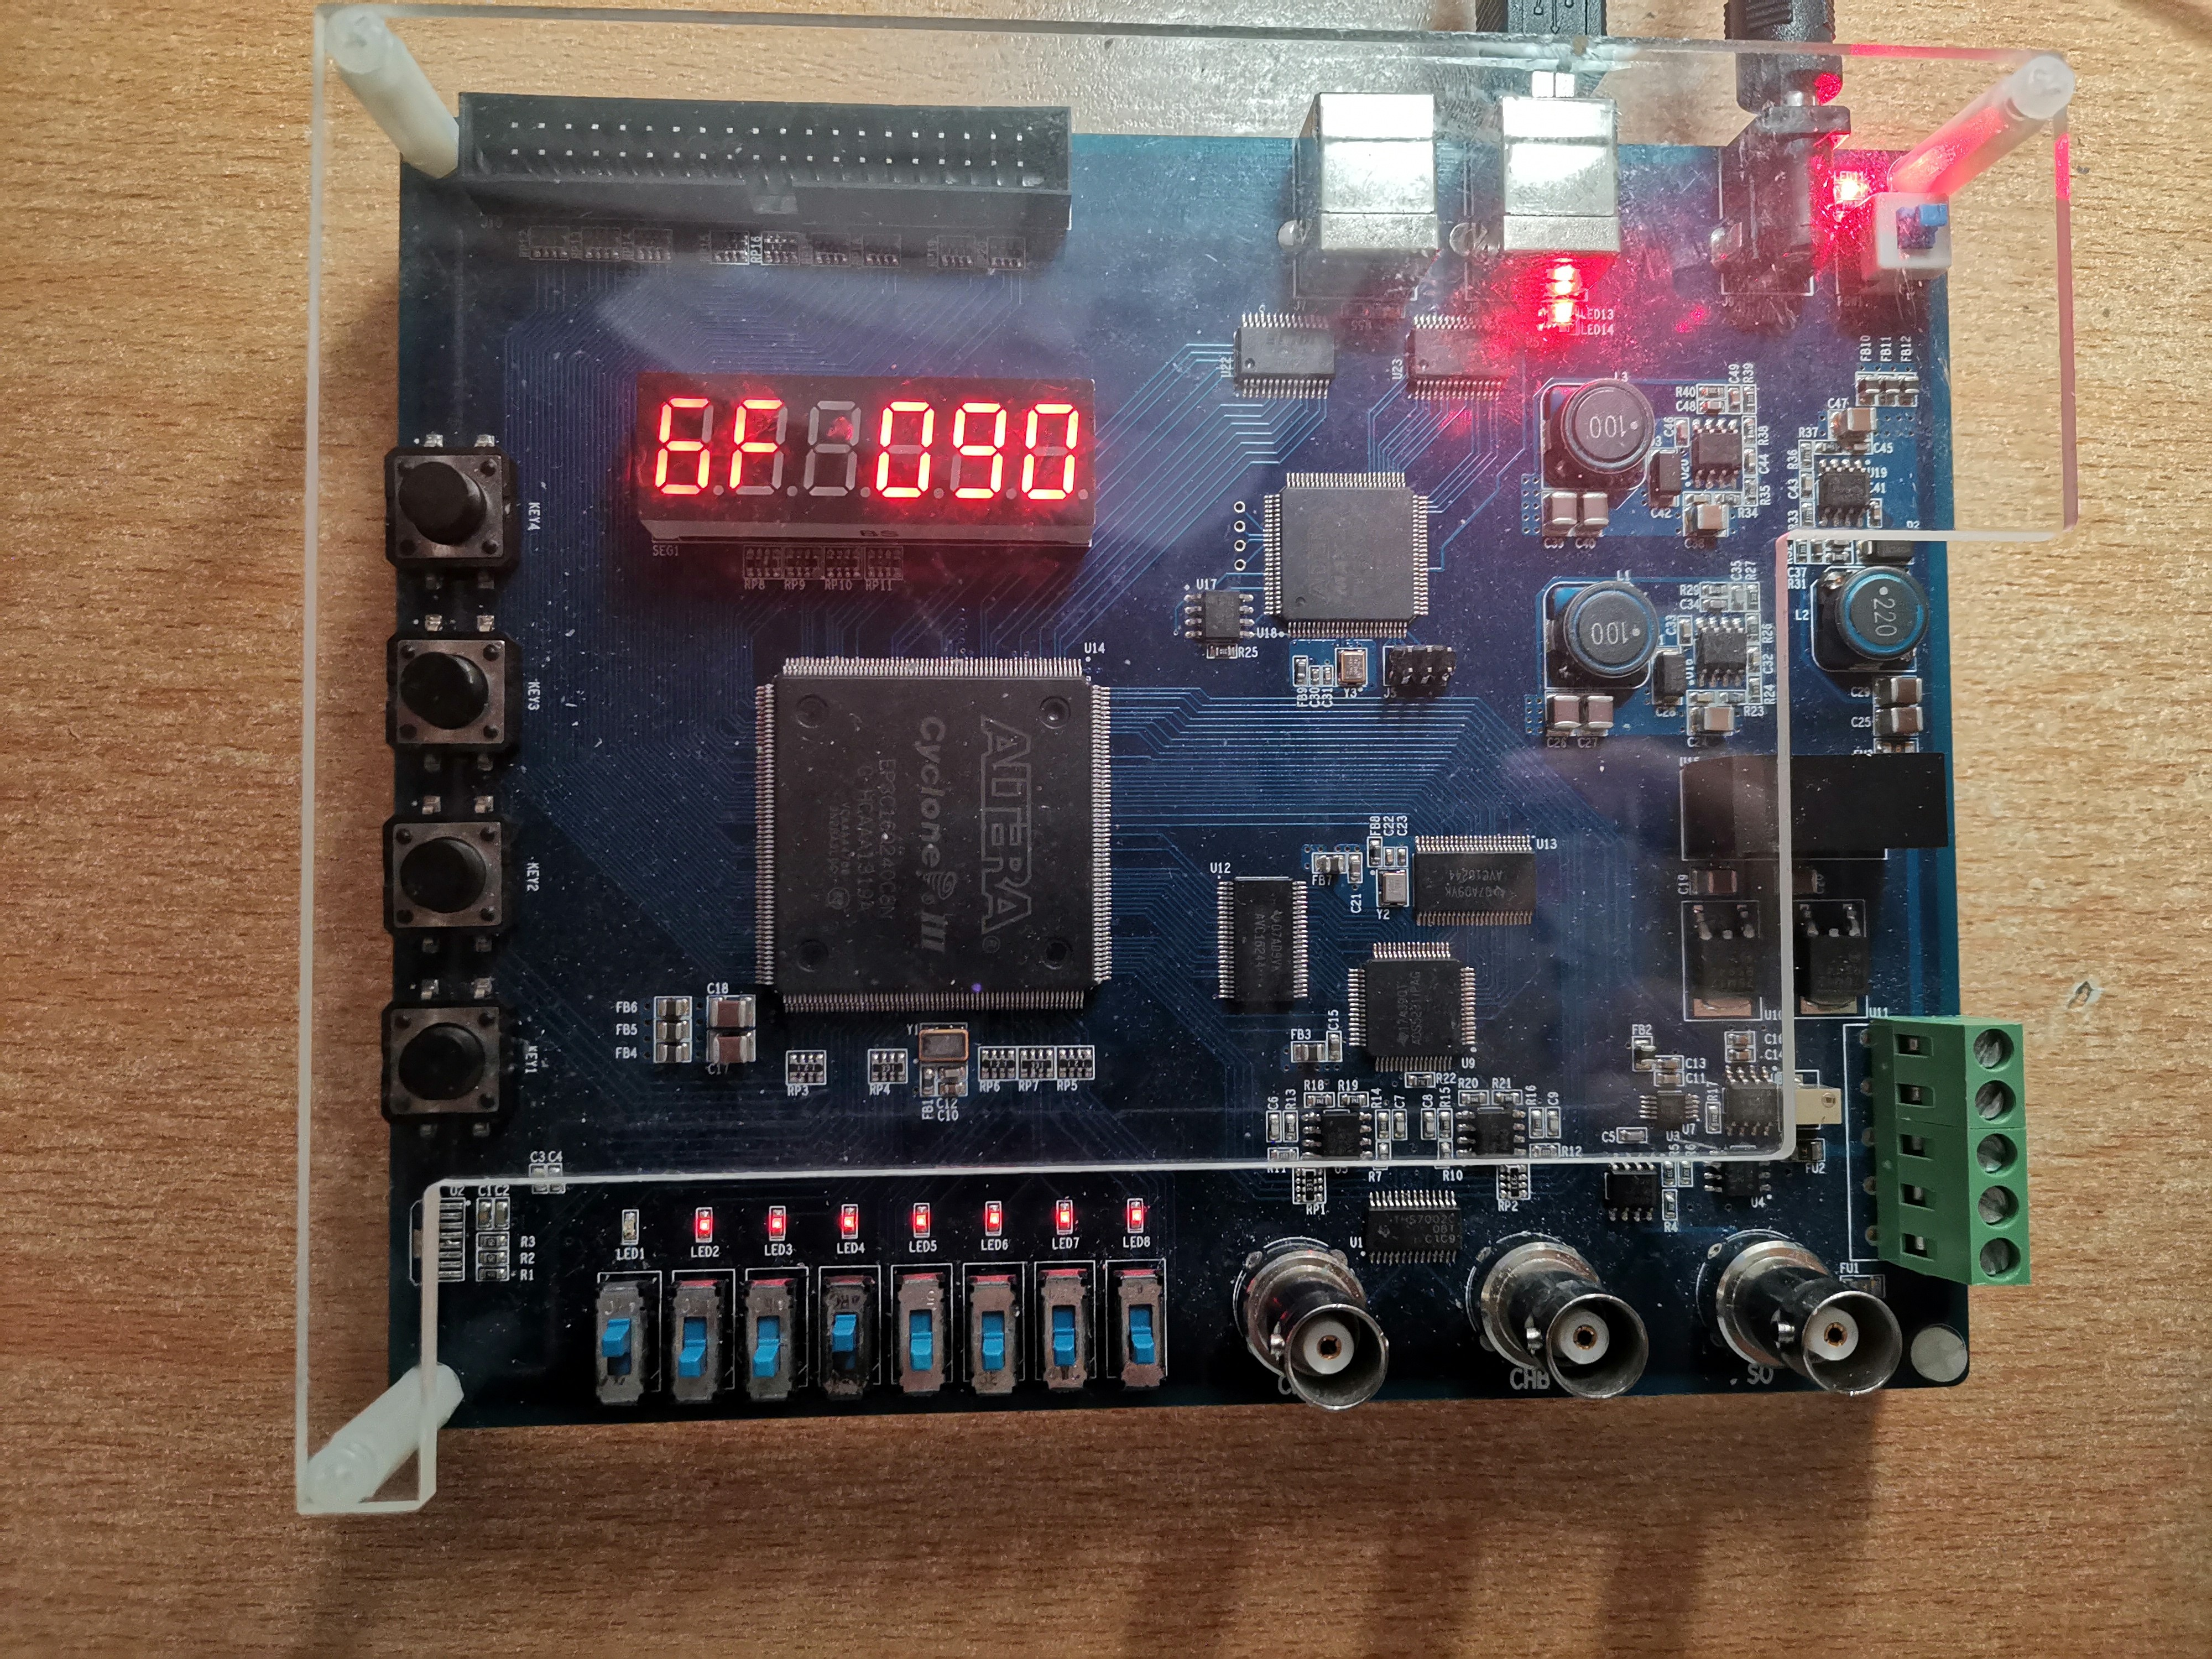
\includegraphics[scale=0.06]{615.jpg}}\hspace{0.3mm}
    \subfigure[15×15=225]{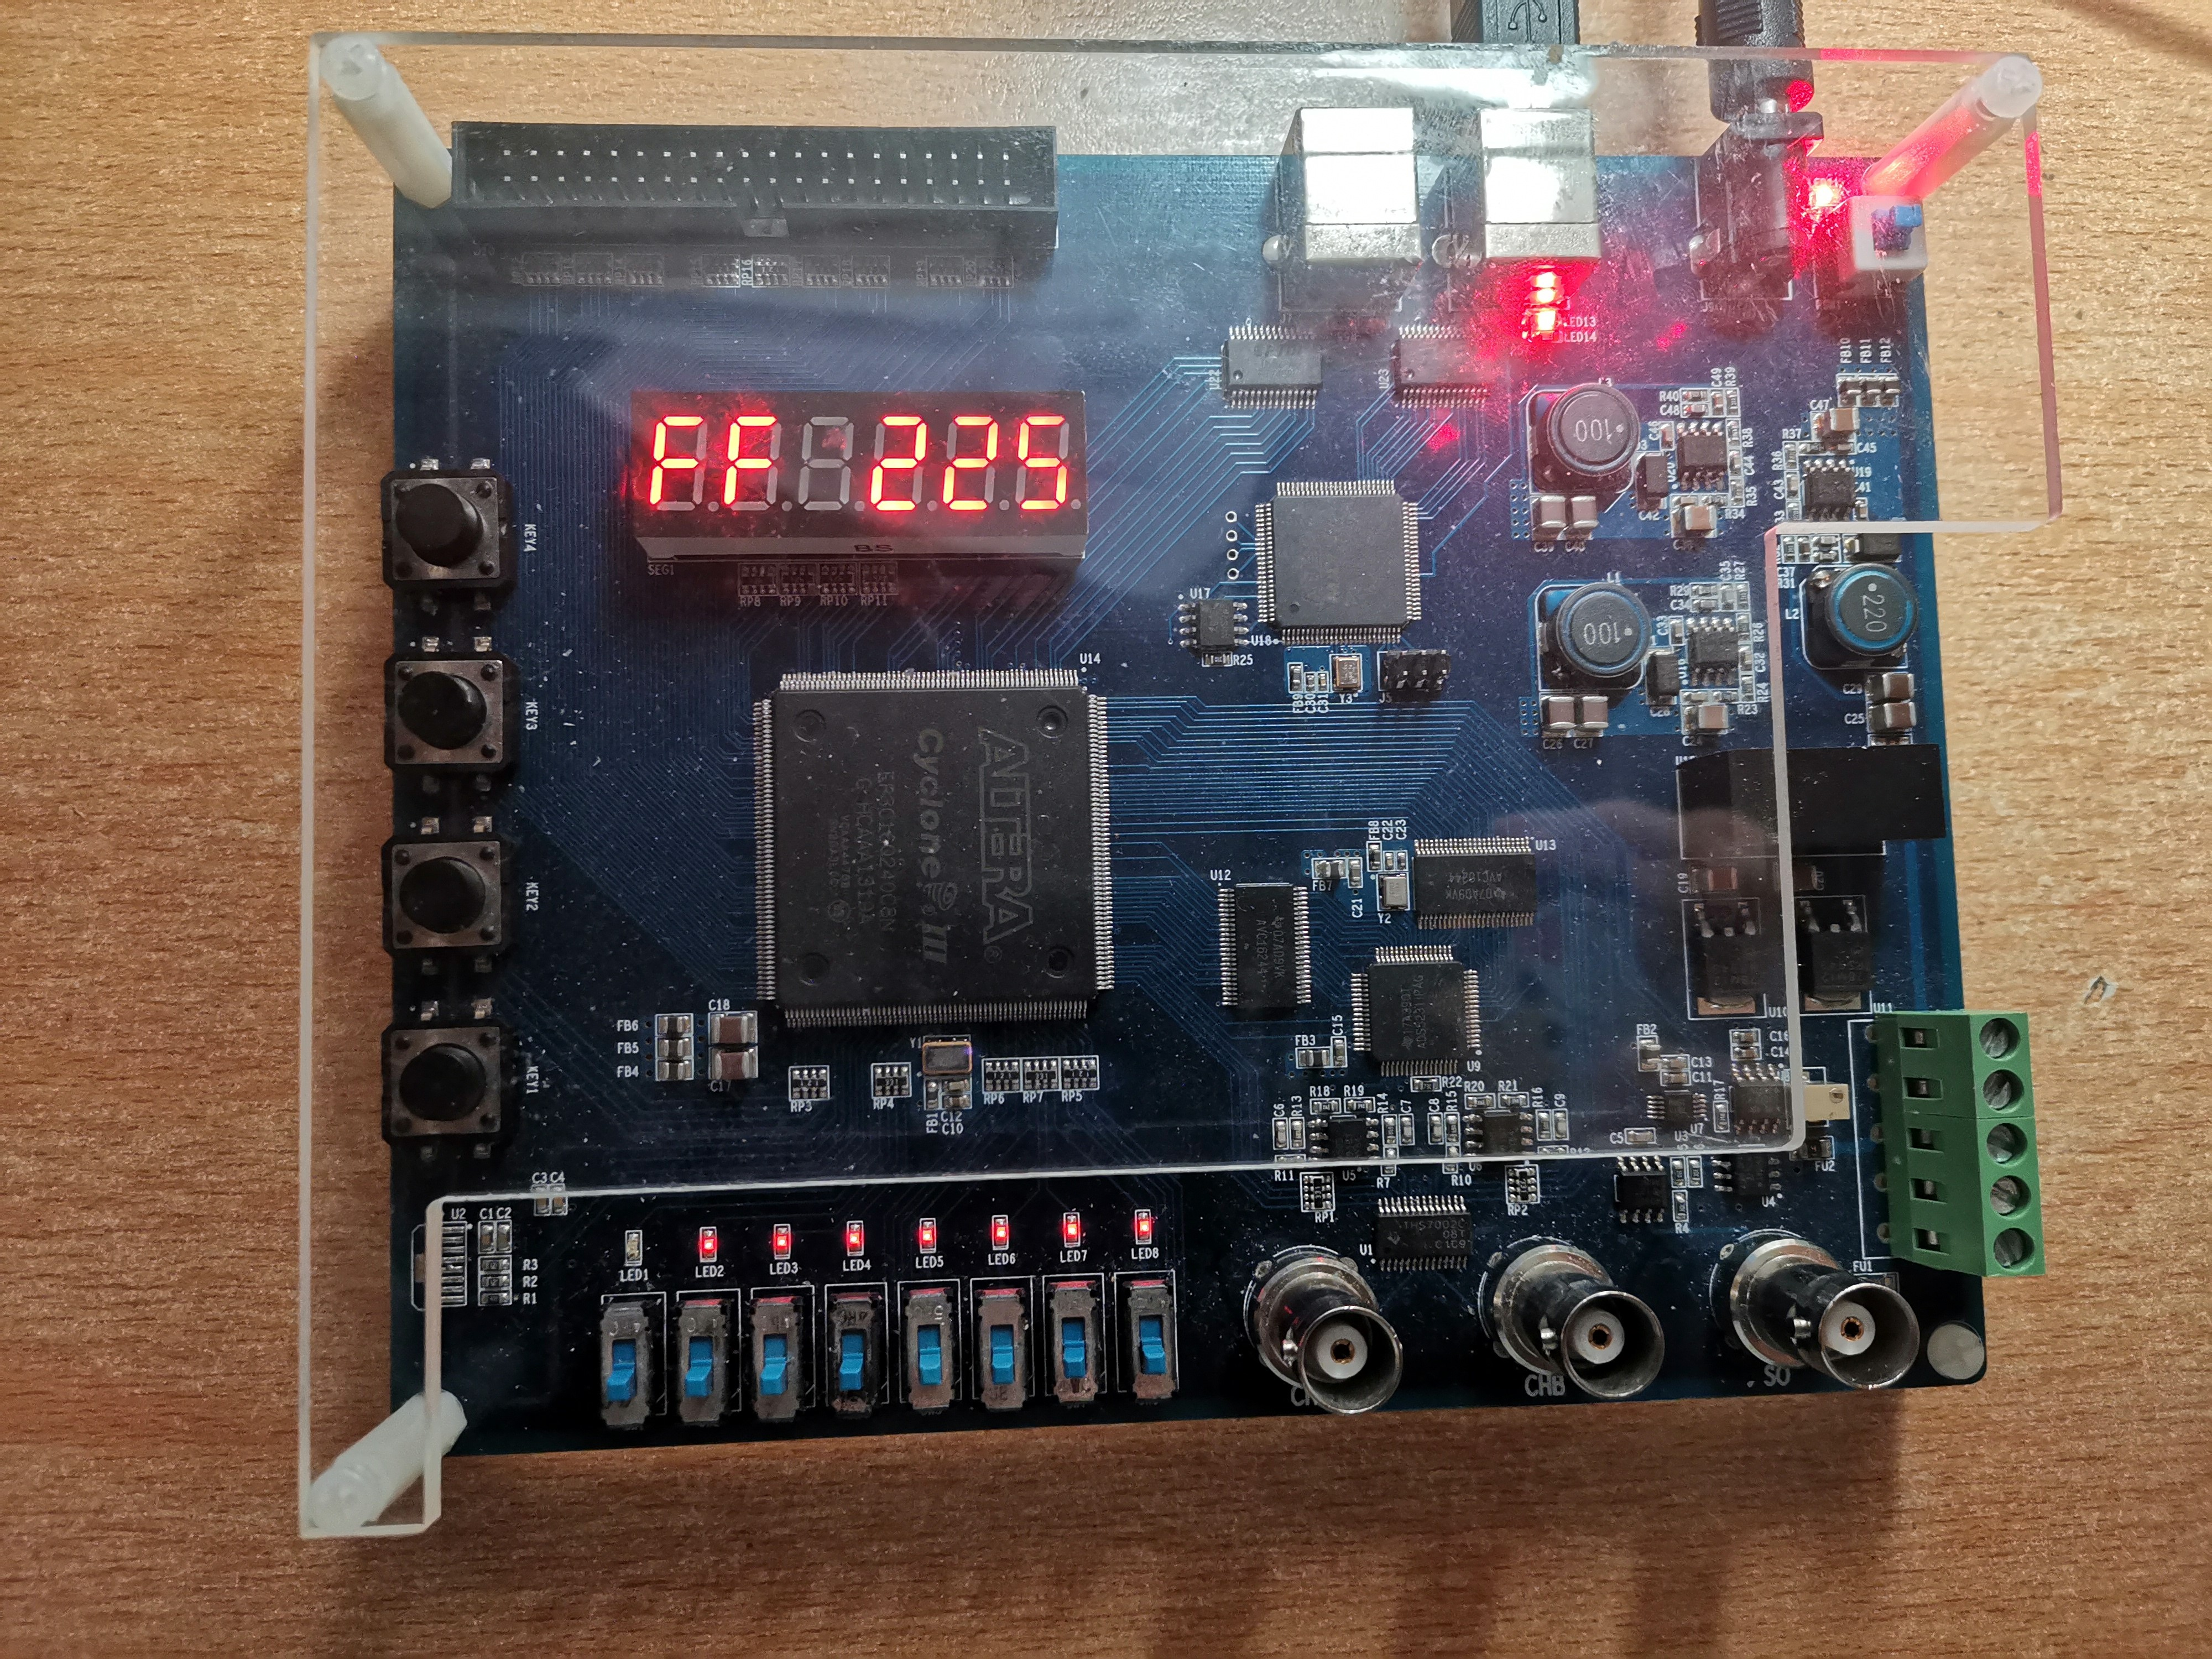
\includegraphics[scale=0.06]{1515.jpg}}\hspace{0.3mm}
    \subfigure[12÷12=1]{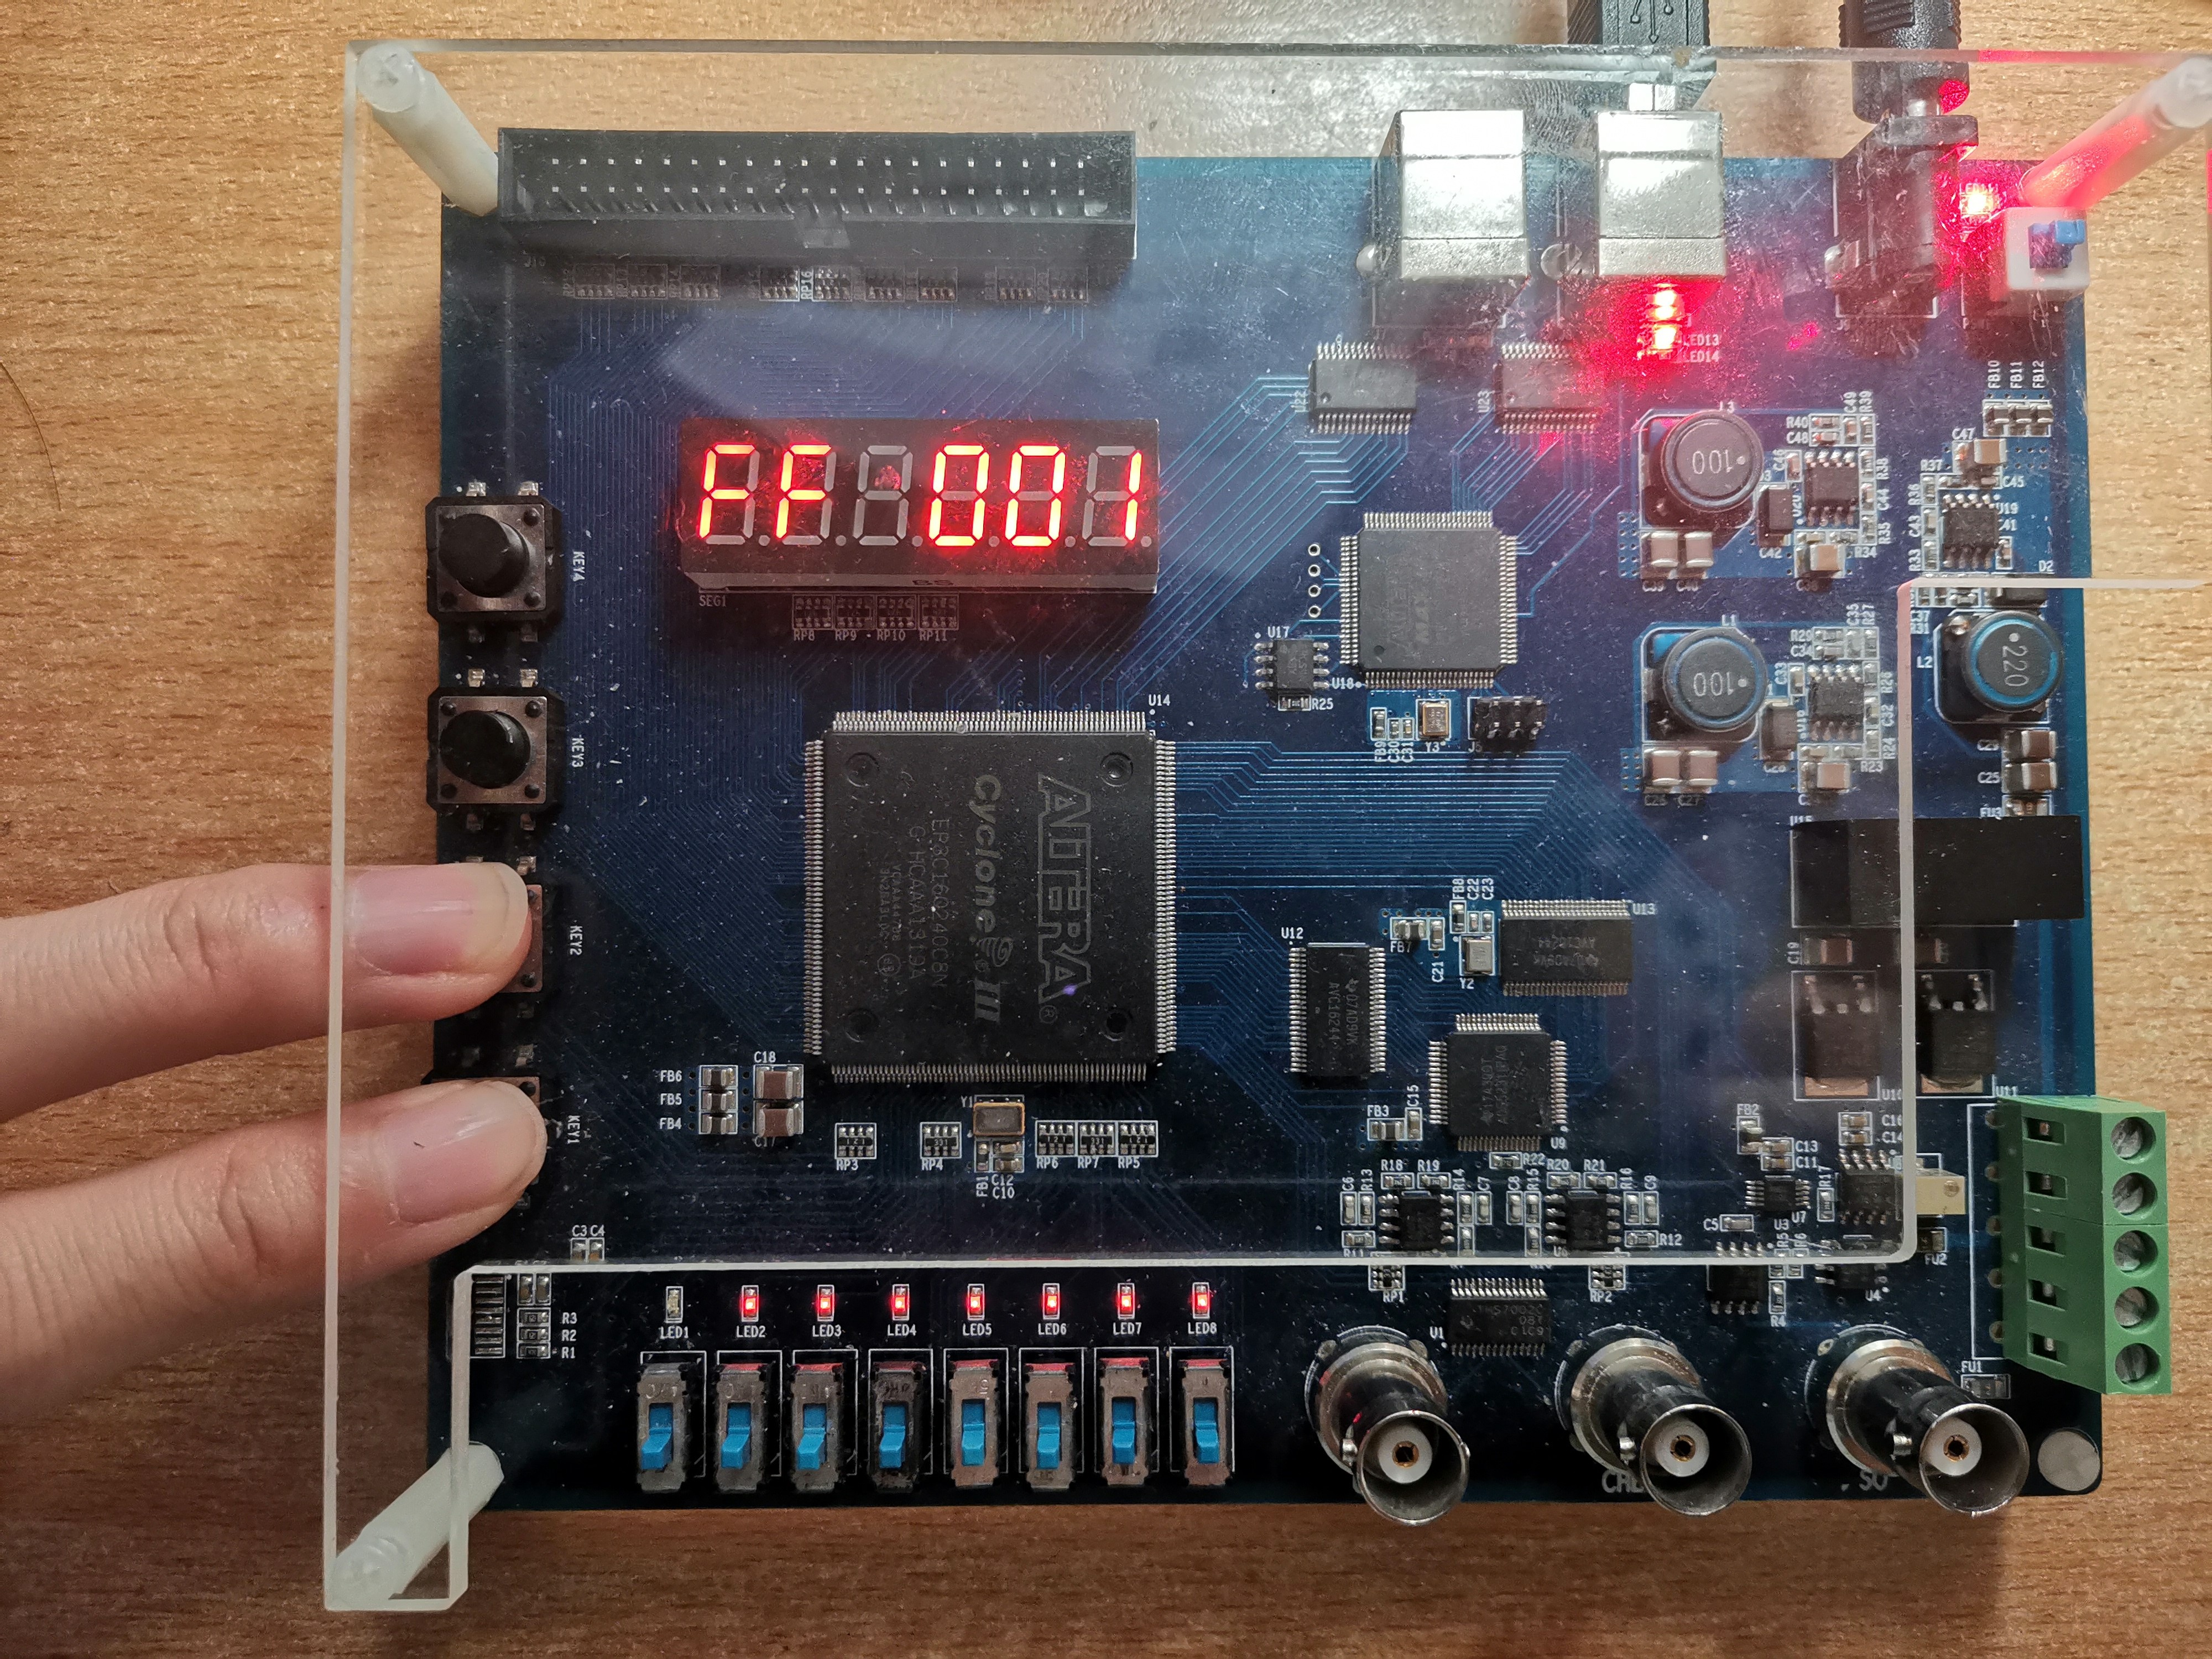
\includegraphics[scale=0.06]{1212.jpg}}\hspace{0.3mm}
    \subfigure[9÷3=3]{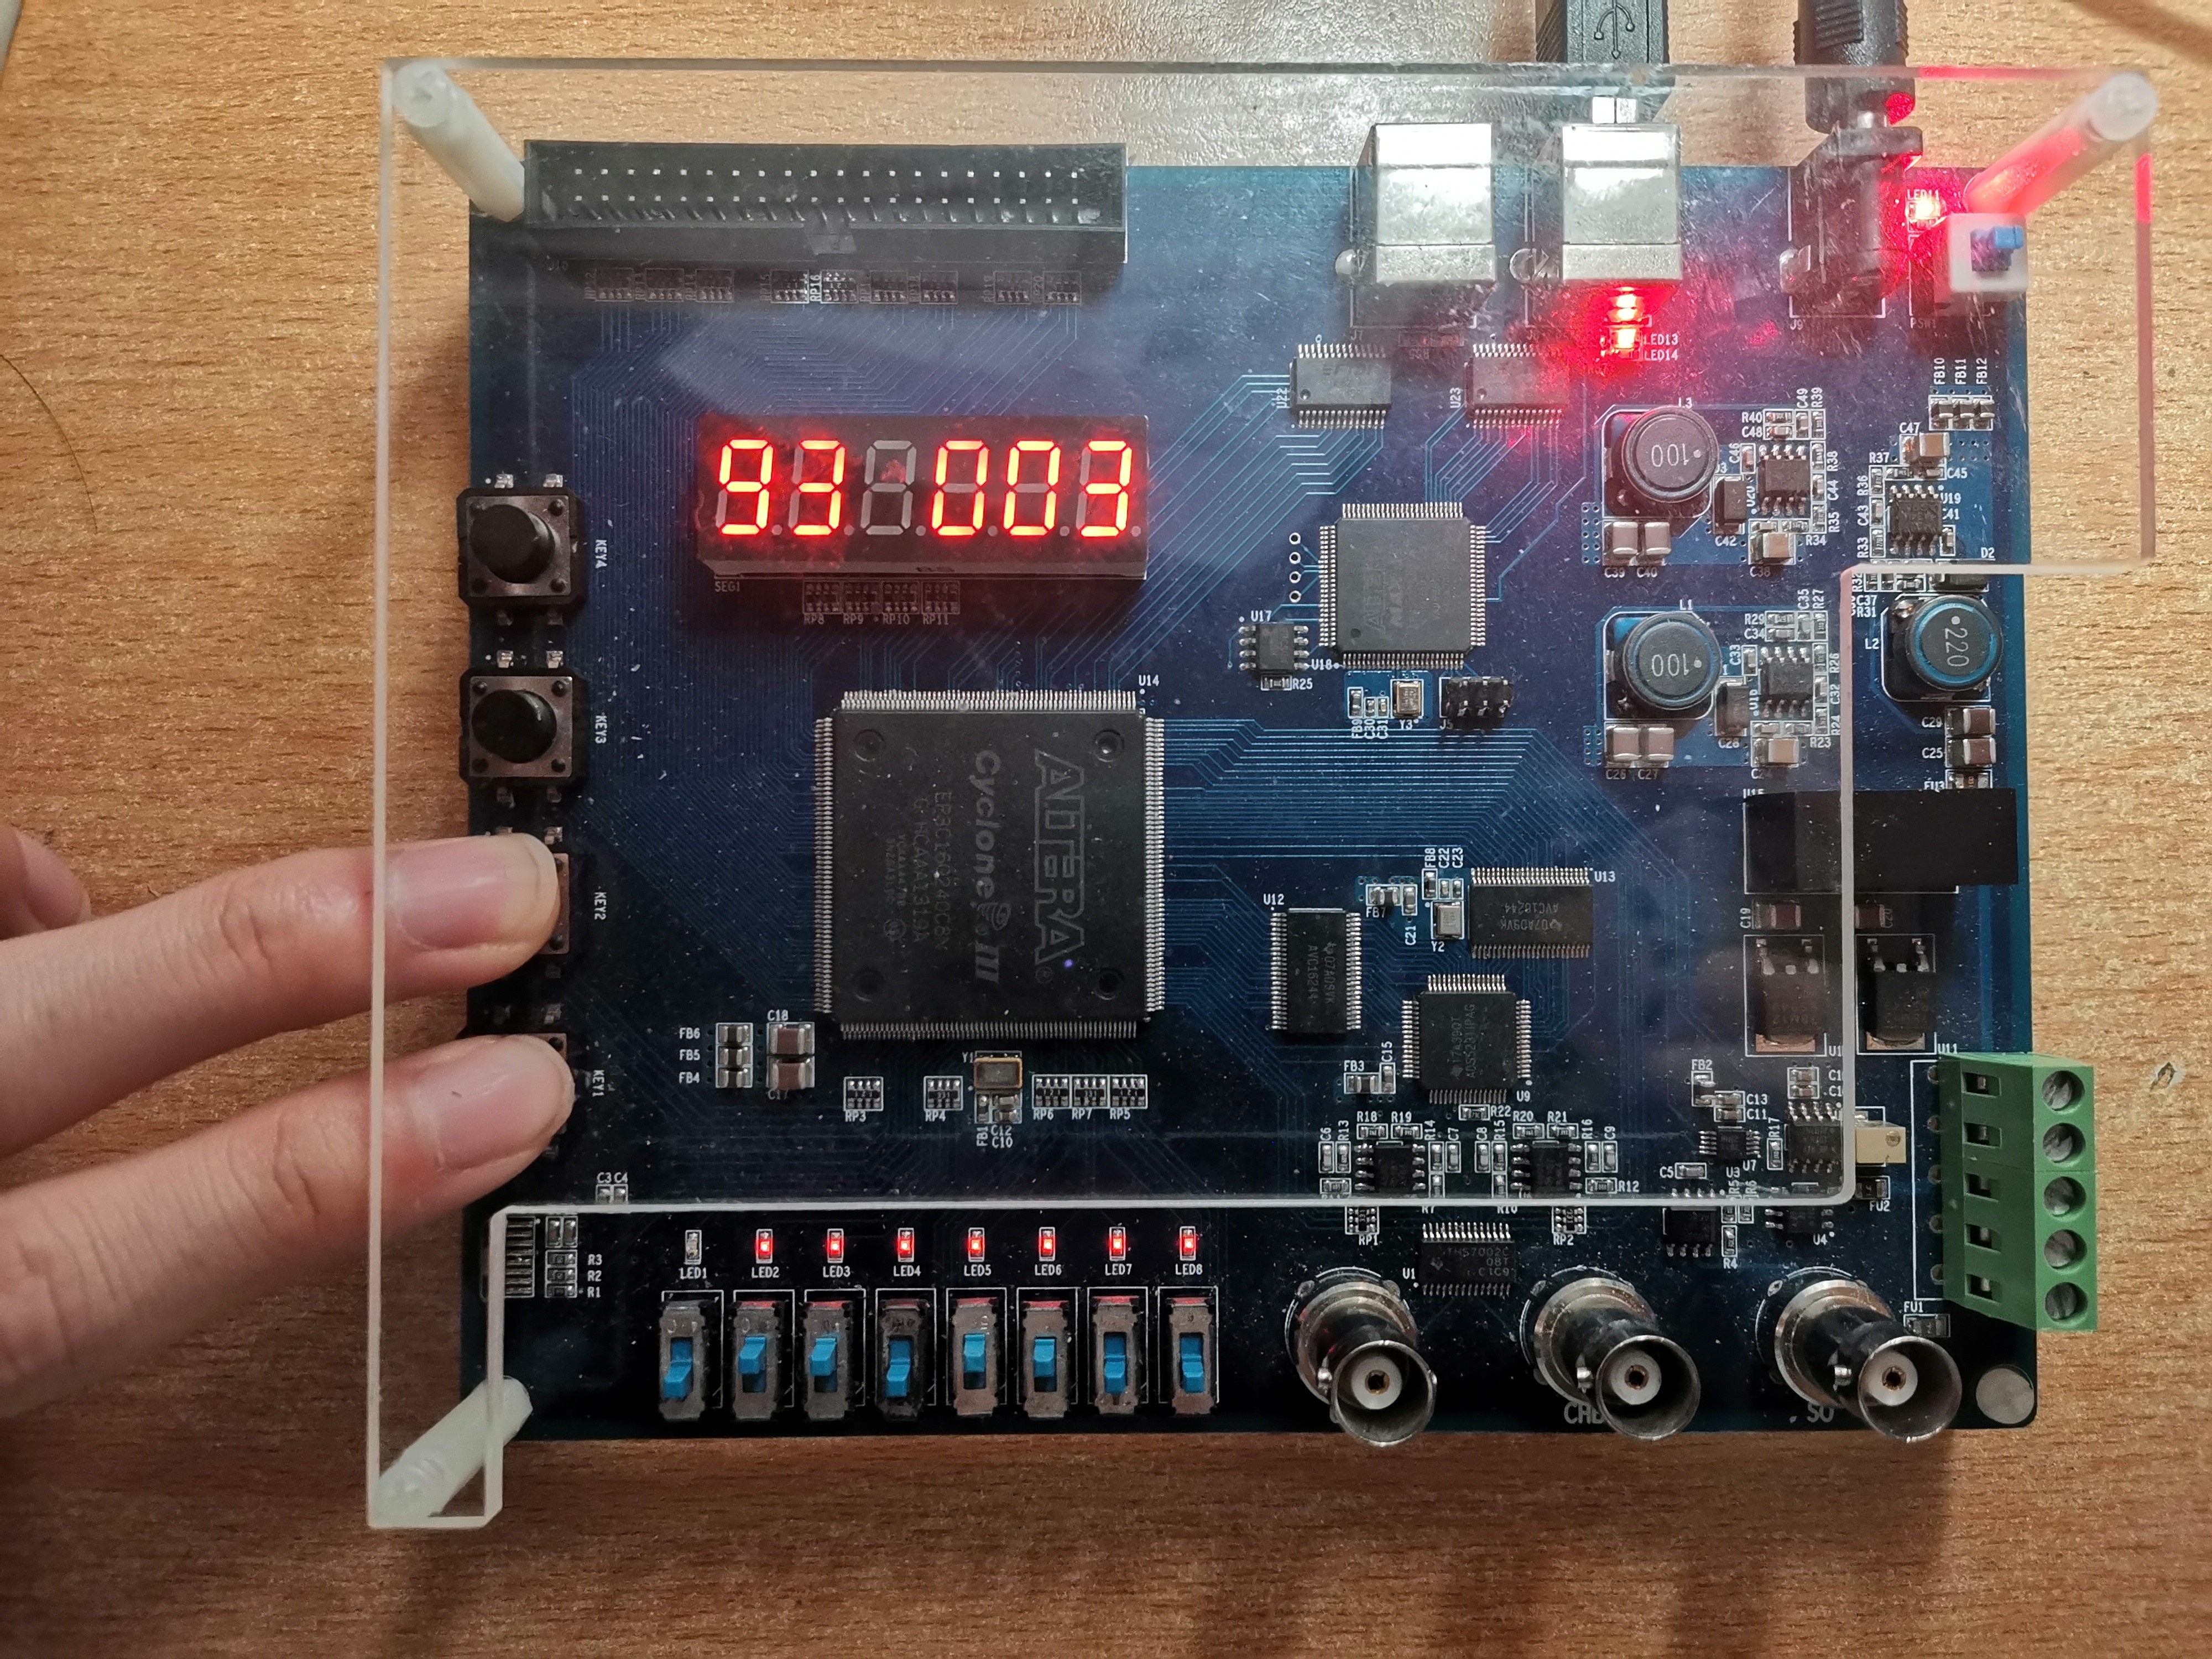
\includegraphics[scale=0.06]{93.jpg}}\hspace{0.3mm}
    \restoregeometry
    }
\end{figure}\par
\section{特别说明}
本实验我实现的附加功能有:\par
1) 同时显示计算数a和b;\par
2) 可以在数码管上显示负号;\par
3) 实现除法.

\section{实验中遇到的困难及其解决}
\paragraph{缺少模块化思维}最开始我在主函数中通过assign语句和always语句接线,但导致的后果是代码写到一半,逻辑已经异常混乱了. 于是我自顶而下开始重新设计,将需要实现的功能一个一个分类并且划分成模块,然后再自底向上实现小模块并在主函数中将各个模块组装,由此写出的代码异常清晰且非常利于维护.
\paragraph{扫描信号的获得}老师上课讲授如何获得分频信号,我据此想设计出根据分频信号变化的计数器,但我将计数器增加写在了分频信号获得的always里面,写成if(CLK\_)count=count+1;导致每一个原始CLK信号的上升沿来临且分频后信号CLK\_处于高电平时,计数器都会自增;这样导致的必然后果是,计数器实际上是根据原始频率计数的,分频信号失去了用处. 如果将获得分频信号和分频信号计数两个模块分开来写,就能有效避免这个问题,这也再一次体现了模块化设计会导致错误率降低的优势.
\paragraph{区分reg和wire}wire适用于连续赋值,相当于硬件电路中的各种物理连接,输入值紧随输出值的变化而变化,于是需要用assign分配赋值. 而reg为寄存器,能够储存过去时态的值,适用于过程语句赋值,它是在运行过程中修改reg的赋值,如边沿触发、电平触发,这样的赋值方式并不是输入输出实时一一对应的,而在于在一定条件下“修改”赋值,也因此,我们只能用always过程块来实现过程语句赋值. 这样,wire和assign,reg和always就构成两个截然不同的变量-使用方法的元组.
\paragraph{显示负号和灭零}开始时,七段译码器只能译码0-f,无法实现更多显示功能,因此,我就尝试设置特殊值:表示负号时,我对于四位的向量赋值-1,但总会出显示错误,后来我才意识到-1实际上就是以补码显示的4'b1111,这样必然会和f成为一个代号,因此需要对原来的向量进行扩容,唯有将向量扩充一位,才能表示出这些特殊的情况.

\paragraph{注意向量的位数}对于向量来说,如果多位向量传参时传递到位数较少的向量上时,长向量会截去头部,可能造成错误. 如乘法时,四位向量乘四位向量,结果是八位向量,如果位数不足够,就可能造成数据的丢失,因此应该时刻注意向量的位数问题,避免出错.

\end{document}
